%%% template.tex
%%%
%%% This LaTeX source document can be used as the basis for your technical
%%% paper or abstract. Intentionally stripped of annotation, the parameters
%%% and commands should be adjusted for your particular paper - title, 
%%% author, article DOI, etc.
%%% The accompanying ``template.annotated.tex'' provides copious annotation
%%% for the commands and parameters found in the source document. (The code
%%% is identical in ``template.tex'' and ``template.annotated.tex.'')

\documentclass[review]{acmsiggraph}

\usepackage{subcaption}
\usepackage{color}

% Reduce the space between subfigures and subfigure captions.
\captionsetup[subfigure]{aboveskip=6pt}
\captionsetup[subfigure]{belowskip=0pt}

\TOGonlineid{33}
\TOGvolume{0}
\TOGnumber{0}
\TOGarticleDOI{1111111.2222222}
\TOGprojectURL{}
\TOGvideoURL{}
\TOGdataURL{}
\TOGcodeURL{}

\title{Painting with Triangles}

\author{Mark D. Benjamin\thanks{e-mail:mdbenjam@princeton.edu} \hspace{10 pt} Princeton Unviersity\\ Adam Finkelstein\thanks{e-mail:af@cs.princeton.edu} \hspace{10 pt} Princeton University\\ Stephen DiVerdi\thanks{e-mail:diverdi@google.com} \hspace{10 pt} Google}
\pdfauthor{Mark D. Benjamin, Adam Finkelstein, Stephen Diverdi}

\keywords{triangle mesh, painting, vector graphics}

%%%%% For comments:
\newcommand{\ignorethis } [1] {}
\newcommand{\smallnote  } [1] {{\small \{#1\}}}
\newcommand{\bignote    } [1] {\begin{quote} \textbf{Note:\ }
                               \slshape #1 \end{quote}}
\newcommand{\todo}[1]{\ignorethis{\textcolor{red}{[{\bf TODO}: #1]}}}
\newcommand{\redund}[1]{#1}

%%%%% For referencing things:
\newcommand{\chapnum    } [1] {\ref{#1}}
\newcommand{\appnum     } [1] {\ref{#1}}
\newcommand{\sectnum    } [1] {\ref{#1}}
\newcommand{\tblnum     } [1] {\ref{#1}}
\newcommand{\fignum     } [1] {\ref{#1}}
\newcommand{\eqnnum     } [1] {\mbox{(\ref{#1})}}
\newcommand{\chap       } [1] {Chapter~\chapnum{#1}}
\newcommand{\chaps      } [1] {Chapters~\chapnum{#1}}
\newcommand{\app        } [1] {Appendix~\appnum{#1}}
\newcommand{\apps       } [1] {Appendices~\appnum{#1}}
\newcommand{\sect       } [1] {Section~\sectnum{#1}}
\newcommand{\sects      } [1] {Sections~\sectnum{#1}}
\newcommand{\tbl        } [1] {Table~\tblnum{#1}}
\newcommand{\tbls       } [1] {Tables~\tblnum{#1}}
\newcommand{\fig        } [1] {Figure~\fignum{#1}}
\newcommand{\figs       } [1] {Figures~\fignum{#1}}
\newcommand{\eqn        } [1] {equation~\eqnnum{#1}}
\newcommand{\eqns       } [1] {equations~\eqnnum{#1}}

%%%%% Latin and language:
%% \newcommand{\etal       }     {\textit{et~al.}} old; not like ACM style
\newcommand{\etal       }     {{et~al.}}
\newcommand{\apriori    }     {\textit{a~priori}}
\newcommand{\aposteriori}     {\textit{a~posteriori}}
\newcommand{\perse      }     {\textit{per~se}}
\newcommand{\cf         }     {\textit{cf.}}
\newcommand{\eg         }     {{e.g.}}
\newcommand{\Eg         }     {{E.g.}}
\newcommand{\ie         }     {{i.e.}}
\newcommand{\Ie         }     {{I.e.}}
\newcommand{\vs         }     {{vs.}}
\newcommand{\naive      }     {{na\"{\i}ve}}

%%%%% Math symbols:
\newcommand{\Identity   }     {\mat{I}}
\newcommand{\Zero       }     {\mathbf{0}}
\newcommand{\Reals      }     {{\textrm{I\kern-0.18em R}}}
\newcommand{\isdefined  }     {\mbox{\hspace{0.5ex}:=\hspace{0.5ex}}}
%\newcommand{\implies    }     {\Longrightarrow}
\newcommand{\texthalf   }     {\ensuremath{\textstyle\frac{1}{2}}}
\newcommand{\half       }     {\ensuremath{\frac{1}{2}}}
\newcommand{\third      }     {\ensuremath{\frac{1}{3}}}
\newcommand{\fourth      }    {\ensuremath{\frac{1}{4}}}

%%%%% Math modifiers:
\renewcommand{\vec      } [1] {{\text{\boldmath $\mathbit{#1}$}}}
\newcommand{\mat        } [1] {{\text{\boldmath $\mathbit{#1}$}}}
\newcommand{\Approx     } [1] {\widetilde{#1}}
\newcommand{\change     } [1] {\mbox{{\footnotesize $\Delta$} \kern-3pt}#1}

%%%%% Math functions:
\newcommand{\Order      } [1] {O(#1)}
\newcommand{\set        } [1] {{\lbrace #1 \rbrace}}
\newcommand{\floor      } [1] {{\lfloor #1 \rfloor}}
\newcommand{\ceil       } [1] {{\lceil  #1 \rceil }}
\newcommand{\inverse    } [1] {{#1}^{-1}}
\newcommand{\transpose  } [1] {{#1}^\mathrm{T}}
\newcommand{\invtransp  } [1] {{#1}^{-\mathrm{T}}}

%%%%% Math functions with small (fixed) and large (expandable) forms:
\newcommand{\abs        } [1] {{| #1 |}}
\newcommand{\Abs        } [1] {{\left| #1 \right|}}
\newcommand{\norm       } [1] {{\| #1 \|}}
\newcommand{\Norm       } [1] {{\left\| #1 \right\|}}
\newcommand{\pnorm      } [2] {\norm{#1}_{#2}}
\newcommand{\Pnorm      } [2] {\Norm{#1}_{#2}}
\newcommand{\inner      } [2] {{\langle {#1} \, | \, {#2} \rangle}}
\newcommand{\Inner      } [2] {{\left\langle \begin{array}{@{}c|c@{}}
                               \displaystyle {#1} & \displaystyle {#2}
                               \end{array} \right\rangle}}


%%%%% Paper-specific stuff:

% reduce hyphenation (slay the hyper hyphenator with 2000)
\pretolerance 800

% These variables are for width and height and gaps in figures:
% set with something like: \setlength{\h}{1cm}
\newlength{\w}
\newlength{\h}
\newlength{\x}


\definecolor{darkred}{rgb}{0.7,0.1,0.1}
\definecolor{darkgreen}{rgb}{0.1,0.7,0.1}
\definecolor{cyan}{rgb}{0.7,0.0,0.7}
\definecolor{dblue}{rgb}{0.2,0.2,0.8}
\newcommand{\Mark}[1]{\textcolor{red}{{\slshape #1}}}
\newcommand{\Adam}[1]{\textcolor{darkgreen}{\textbf{Adam:} {\slshape #1}}}
\newcommand{\Steve}[1]{\textcolor{cyan}{\textbf{Steve:} {\slshape #1}}}
\newcommand{\note}[1]{\textcolor{darkgreen}{\textbf{Note:} {\slshape #1}}}
\newcommand{\modified}[1]{#1}%\textcolor{darkgreen}{{#1}}}

\newcommand{\argmin}{\operatornamewithlimits{argmin}}

\newcommand{\mytilde}{\raise.17ex\hbox{$\scriptstyle\sim$}}


\begin{document}

\teaser{
  \setlength{\w}{0.33\textwidth}
  \centering
  
\includegraphics[width=\w]{images/rainbow3}
  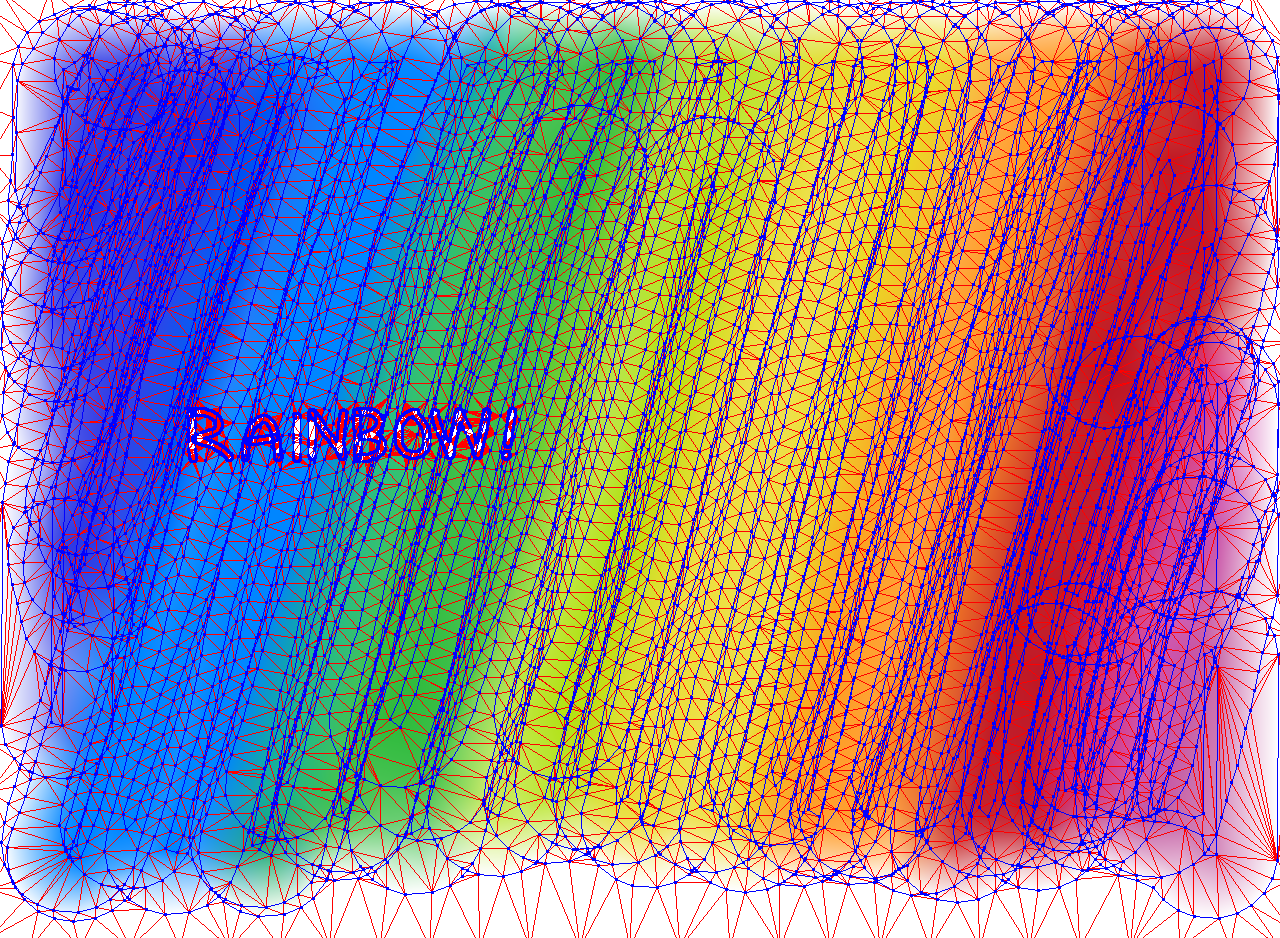
\includegraphics[width=\w]{images/rainbow3_tri}
  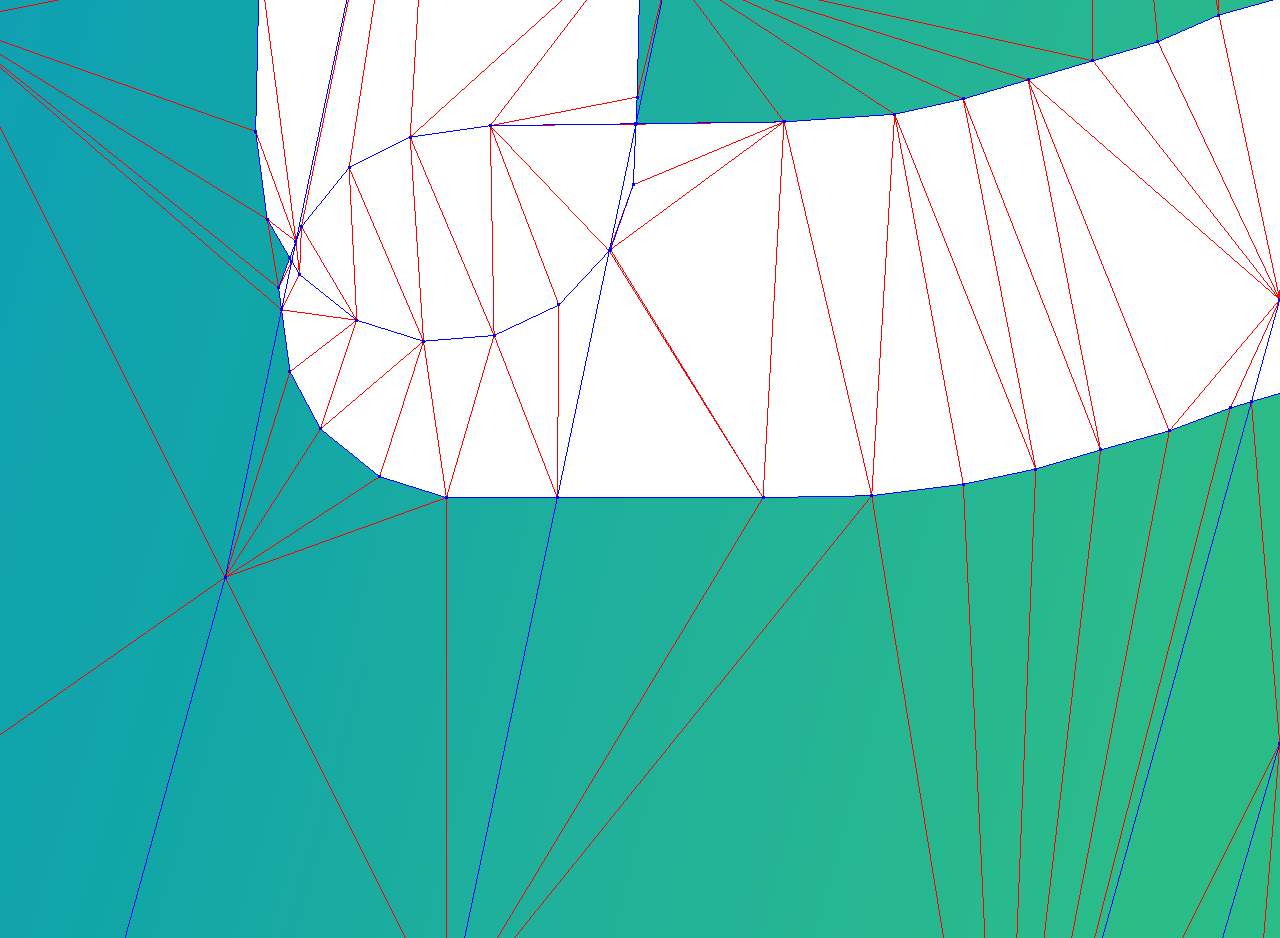
\includegraphics[width=\w]{images/rainbow3_zoom3}
  \caption{\emph{Left:} A vector painting made in the system exhibits both smooth gradients painted by soft brushes as well as infinitely sharp boundaries painted by hard brushes. \emph{Middle:} The painting is represented by a planar triangle mesh. \emph{Right:} Closeup on the bottom of the letter B highlights both the sharp boundaries on the white region and smooth gradient from blue to green in the background.}
  \label{fig:teaser}
}

\maketitle

\begin{abstract}
Although vector graphics offer a number of benefits, conventional vector painting programs
do not allow an artist to use traditional (digital) painting techniques. 
% \note{really?}
We propose a new algorithm that translates a
user's mouse motion into a triangle mesh representation. This triangle mesh can then be composited onto
a canvas containing an existing mesh representation of the previous strokes. 
This representation allows the algorithm to render solid colors and linear
gradients. It also enables painting at any resolution. This gives artists the opportunity to create complex,
multi-scale drawings with gradients while avoiding artifacts.  

\end{abstract}

\ignorethis{
\begin{CRcatlist}
  \CRcat{I.3.4}{Computer Graphics}{Graphics Utilities}{Paint systems}
  \CRcat{I.3.6}{Computer Graphics}{Methodology and Techniques}{Graphics data structures and data types}
\end{CRcatlist}
}

\keywordlist

%% Use this only if you're preparing a technical paper to be published in the 
%% ACM 'Transactions on Graphics' journal.

\TOGlinkslist

%% Required for all content. 

\copyrightspace

\section{Introduction}

All computer painting programs must store data through rasterization or vectorization. 
However, traditional computer painting programs take inputs of the same type as the stored data. 
For example, programs like Adobe Photoshop and GIMP
allow a user to paint how he would on a physical medium. By letting the mouse act as
a brush, a user may color individual pixels on the screen. By contrast, programs like 
Adobe Illustrator and Inkscape let a user paint
using geometric primitives such as lines and B\'{e}zier curves. The program then stores
these geometric primitives in order to render the drawing. Although using vector graphics
is likely less intuitive, it has some distinct advantages including a compact
representation, infinite resolution, and easier manipulation.

In this paper we introduce a system which  
uses a different representation than traditional raster or vector graphics.
The system uses a triangle mesh to store the data of the painting.
Since triangles are a geometric primitive used in vector graphics this approach achieves the
same advantages traditional vector graphics have. However, the representation allows the
user to paint with vector graphics without dealing directly with the underlying implementation.

In order to paint in our program the user simply drags his mouse on the screen to make
strokes akin to the process in a raster graphics program. Upon mouse-up the stroke is
converted to our underlying triangle mesh representation. In this way a user may paint using
vector graphics without worrying about the representation.

This procedure allows painting at any scale. A user can make large strokes
while zoomed out and then zoom in to make fine details. All of this can happen without
loss of quality since the data is stored using triangles instead of pixels, which can represent sharp boundaries at any orientation.  Furthermore, the use of smooth shading when rendering the triangles allows for vector representation of gradient effects.  We take advantage of this feature to create soft, airbrush-like strokes, which are difficult to create in vector drawing software.

To transform a user's mouse inputs to a triangle mesh,
the system uses a combination of rasterization and marching squares to
find stroke contours. From the contour it performs a Delaunay triangulation
and then merges this triangulation
of the new stroke with the triangle mesh of the existing canvas. This process yields
a new canvas with the combined strokes.

The system reduces the barrier to creating vector graphics by enabling a painting-like interface, with support for sharp and smooth edges. This in turn allows 
artists to focus on the painting and not the way in which they paint, while still 
getting the benefits of vector graphics. We demonstrate our method by creating digital paintings with a 
range of effects and resolutions, including zoom factors of up to 500,000:1 which implies an effective 
resolution equivalent to an image with more than $10^{17}$ pixels.

\section{Related Work}

Previous work has focused on converting images into vector graphics to take advantage of the
efficient storage, easy editing, and infinite resolution it provides. For example the method of
Lecot and L\'{e}vy~\shortcite{lecot:ARD:2006}
minimizes an energy function to segment an image into a number of regions that are bounded
by cubic splines and filled with solid colors or gradients. A different approach by Lai~\etal~\shortcite{Lai:2009:ATG:1531326.1531391} 
automatically creates gradient meshes with support for holes. 
Our work builds on the representation introduced by
Liao~\etal~\shortcite{10.1109/TVCG.2012.76}, who showed that
a photo can be converted into a triangle mesh.
They demonstrated that natural images can be concisely represented
by triangles, using mesh simplification, and that
various image editing operations can be applied in this representation,
including an abstraction technique similar to that of 
DeCarlo and Santella~\shortcite{DeCarlo:2002:SAP:566654.566650}.
In principle, one could create a digital painting in a conventional
program and then use one of these approaches to convert to a vector
representation. In contrast our paper shows how to paint directly
in this representation, offering several advantages including
efficiency and the ability to handle imagery with enormously
higher effective resolution.
% All three of these can convert images into
% a vector representation, yet none of them allow a user to create a painting in the vector medium.


Other work has proposed novel vector graphic data structures. For example 
Frisken~\etal~\shortcite{Frisken:2000:ASD:344779.344899}
introduced Adaptively Sampled Distance Fields (ADFs), which specify a signed distance function to a surface in 3D
(or a curve in the plane).
%
Rendering the shape requires sampling the function to determine whether or not a pixel is on the shape.
A quadtree accompanies the distance function to specify where higher sampling rates are necessary. The method of Bremer~\etal~\shortcite{Bremer:2001:VCM}
further describes how ADFs can be created and used. However, it remains unclear how ADFs might be used in a general
painting program where strokes with solid colors and gradients are composited on top of one another.

\begin{figure}
    \centering
        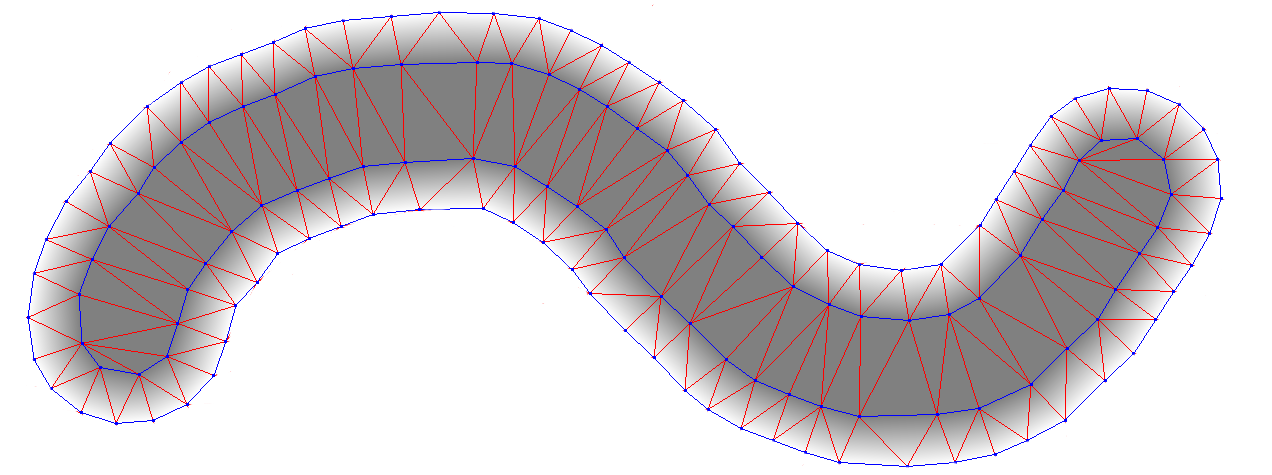
\includegraphics[width=\columnwidth]{images/stroke}
    \caption{Example smooth stroke triangulation. Blue segments are boundary edges, and small blue squares denote
    mesh vertices.}
    \label{fig:stroke}
\end{figure}

There have been a few projects that enable painting directly with vector data.  Most similar is the work of DiVerdi et al.~\shortcite{diverdi2012,diverdi2013}, which uses many polygonal paint splats to create a watercolor-like effect.  These arbitrary polygons are costly to render however, and ``smooth'' effects are only created via many overlapping transparent polygons, which results in a very large amount of geometry. The method of Ando and Tsuruno~\shortcite{ando2010} also uses a dynamic vector representation for their 2D fluid simulation to create marbling patterns stored as B\'{e}zier silhouettes.  They developed a simulation that adaptively updates the B\'{e}zier to maintain nice contours, but the complexity of the document quickly grows too large to compute interactively.  Finally, Asente and Carr~\shortcite{asente2013} implemented a feature in Adobe Illustrator to create contour gradients from shapes, which fill the shapes with small patches of linear gradients to create a bevel-like effect.  Contour gradients can be used to control opacity to create soft strokes, but each stroke must be stored as a separate (aggregate) object rather than a single flattened canvas representation.

Another line of research has explored entirely new ways of painting.
Orzan~\etal~\shortcite{Orzan:2008:DCV:1360612.1360691}
introduced \emph{diffusion curves} --
a new painting technique where artists specify edges and colors for those edges. Their system
then solves a Poisson equation to diffuse the colors between boundary conditions specified at the edges.
Similarly the method of McCann and Pollard~\shortcite{McCann:2008:RGP:1360612.1360692}
lets artists paint in the gradient domain. Both of these approaches yield creative new aesthetic ranges 
beyond what is straightforward in the traditional pixel-based painting model. Nevertheless,
they represent a new painting metaphor for the artist, rather than a vectorized version of the conventional
digital painting approach familiar to artists.

Work has also been done in multi-resolution painting using raster graphics. The method of Berman~\etal~\shortcite{Berman:1994:MPC:192161.192181}
stores image information in a quadtree so that different parts of the image can have different levels of detail.
This means the image effectively has an infinite level of detail, yet since it is stored in raster form
there are still limitations. For example a stroke painted at coarse detail will still look blurry when
zoomed in. The strokes are limited to the resolution they are painted at. Similarly the method of Carr and Hart~\shortcite{Carr:2004:PD:1186562.1015809}
also allows the development of multi-resolution images using rasters, and as such suffers from the
same limitations. Another multi-resolution approach by Perlin and Velho~\shortcite{Perlin:1995:LPP:218380.218437} uses
procedural textures to avoid any fundamental limit on resolution. Although useful,
generating procedural textures can be difficult for artists.

Our work builds on these findings. However, our goal is to enable artists to create vector
graphics through standard painting techniques without having to consider the underlying representation.
\ignorethis{
We start from the triangle mesh structure described by Liao~\etal~\shortcite{10.1109/TVCG.2012.76} to build a painting program
where the triangle mesh is created while the artists lays down strokes. 
}

\begin{figure}
    \centering
        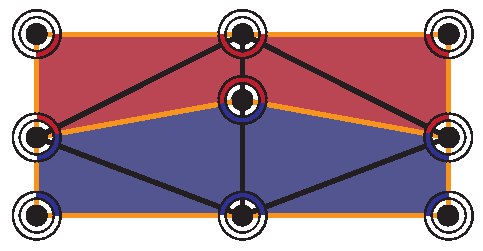
\includegraphics[width=0.4\textwidth]{images/colorarcsfinal}
    \caption{Color arcs. Orange lines are boundary edges, and together with black lines form the triangle
    mesh. Each point is given more or more color arcs, 
    which stores the color of triangle corners in that angular range.
    Points in the middle row have red arcs on top and blue below,
    yielding triangles with those colors, separated by a hard boundary.}
    \label{fig:arcs}
\end{figure}

\section{The Canvas Model}
The data necessary to render the painting resides in the canvas. However, the canvas contains more than just
a triangle mesh, and understanding the underlying data structures is important for 
understanding the rest of the algorithm.

\subsection{Triangle Mesh}
When a user paints, he generates points that are stored on the canvas. These points are
connected to form a triangle mesh. In every triangle the vertices are colored to either
produce a solid color or a linear gradient. In fact a given point that is part of
multiple triangles can take on different colors in each triangle. Note that although
the points are persistent as the canvas is updated, the triangles are not.  
That is, triangulation of the mesh points is not unique, and different, equivalent triangulations may 
be used throughout the painting process.
Thus, we refer to them as ``mesh points'' rather than ``vertices'' (which implies a particular graph
structure).

\subsection{Boundary Edges}
Although the triangles may change over time, they must abide by constraints we call
\emph{boundary edges}, each of which connects a pair of points and specifies that no triangle
can cross it. Like mesh points, boundary edges are persistent. 
%
So as new triangles are created by the triangulation algorithm, they
may never cross a boundary edge.  
This partially restricts the set of valid triangulations of the points.  Figure~\ref{fig:stroke} shows boundary edges for a soft  stroke.

\begin{figure}[t]
    \centering
        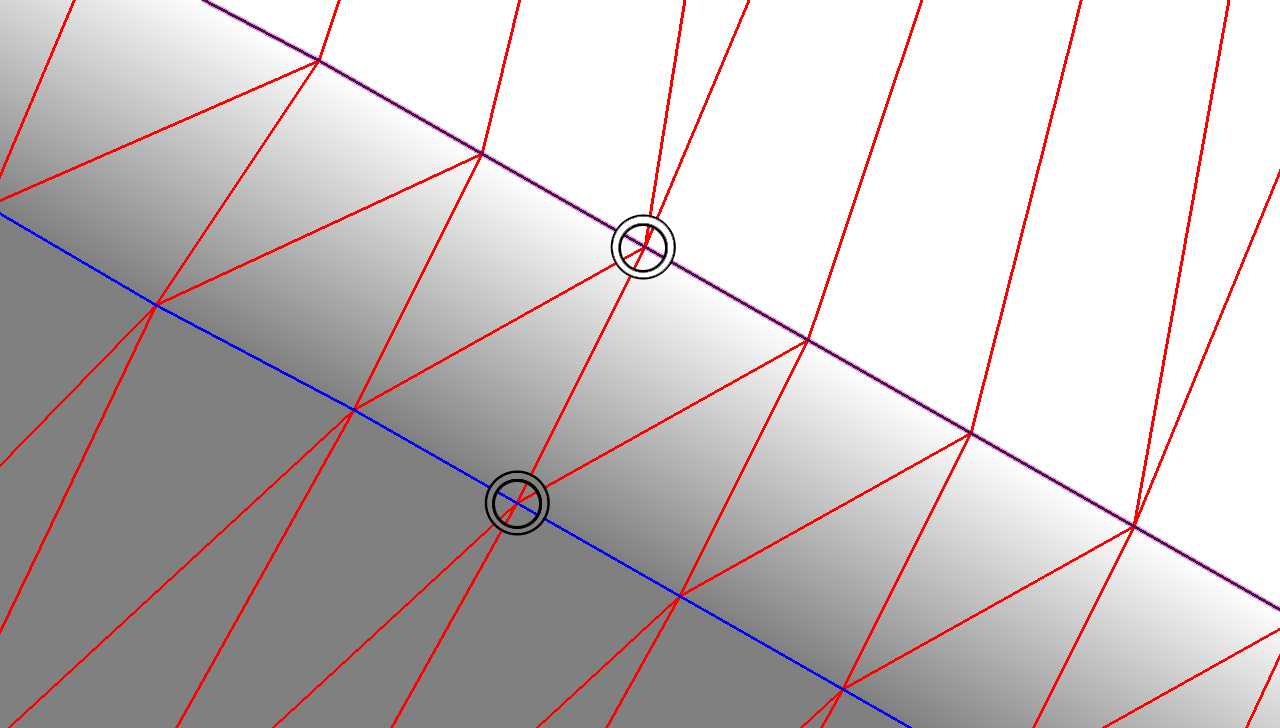
\includegraphics[width=0.5\textwidth]{images/gradientarcs}
    \caption{A close look at a gradient stroke. The blue edges are boundaries where
    the points have gray color arcs as shown. The purple edges are boundaries where
    the points have transparent gray color arcs. This gives triangles connecting the two boundaries
    a linear gradient from gray to white.}
    \label{fig:softarcs}
\end{figure}

\subsection{Color Arcs}
Since triangles are not persistent they cannot store color data.
Storing colors in points works well when the color is the same for all triangles connected
to that point. However, when a point lies on a sharp boundary it may take on different colors in
triangles on either side of the boundary. The need for the same point to take on different
colors in different triangles lead to the development of color arcs (see Figure~\ref{fig:arcs}).

A color arc has three components: a start direction, an end direction, and a color. 
Determining the color of a vertex in a given triangle requires two steps. First,
the vector from the point to the centroid of the triangle is calculated. Second,
the color arc is found which contains this vector. Containing the vector means one must turn
clockwise from the starting direction to reach it and counter-clockwise from the ending direction.
The point takes on the color of the arc in which the vector from the point to the centroid resides.

A point may have more than one color arc, and they must satisfy three conditions. First, they must be disjoint. Second,
they must cover all $2\pi$ radians around the point. These first two conditions ensure that for any
triangle a point will take on exactly one color. Third, the start and end vectors must align
with boundary edges. This condition makes all colors and gradients emanate from boundaries.

\subsection{Rendering}
Once the triangle mesh has been generated it is simple to render. In each triangle the vertices
take on a given color based on their color arcs and the centroid of the triangle. If the three
vertices in the triangle take on the same color value then the triangle will be flat shaded. If instead the 
vertices take on different color values then there will be a gradient over the triangle.

Since the conditions on color arcs make colors emanate from boundaries it is easy to create regions (e.g. a brush stroke boundary)
containing either a solid color or linear gradient. A region will have a solid color (e.g. a hard brush stroke) if the
boundaries that surround it all take on the same color. If instead a region is surrounded by
two boundaries, one which has a given color and the other which has a transparent version of that color
then there will be a linear gradient in that region between the two boundaries (e.g. a soft brush stroke).
Figure~\ref{fig:softarcs} shows the color arcs on such a soft stroke.

\section{Triangulating Strokes}

Here we consider how to convert a user's cursor motion into a triangle-mesh representation
of their stroke. This is done in two steps. First, the stroke is rasterized and the
contour is extracted from the raster. Second, the contour is converted into points and
boundaries and triangulated.

\subsection{Converting Strokes to Contours}
A set of contours define the outline of a stroke. For simply connected strokes, those without holes, 
one contour describes the whole stroke. However, strokes with holes, such as a circle or 
figure-eight, will have more than one contour.
Converting a user's mouse motion into a set of contours requires two steps.
First, the user's mouse movements are captured by a set of polygons which can be
rendered to yield a rasterized version of the stroke.
Second, to obtain the contours the stroke is rasterized in black and marching squares~\cite{lorensen1987}
is used to extract iso-contours of 50\% gray. This returns a very dense set of points 
which we reduce through a pruning process to
get a sparse but accurate representation of the contour.


% Adam and Steve should we talk about how anti-aliasing + marching squares can achieve sub-pixel
% resolution?

% Note that despite the reliance on rasterization it is still possible by using
% anti-aliasing and certain brushes to get sub-pixel resolution.

\subsection{Converting Contours to Triangles}
The contour contains two important pieces of information. First, it describes all of the points of the stroke.
Second, segments connecting adjacent points describe the boundaries of the stroke. 
A triangle mesh must contain all the points and stay
within the boundaries. 
For example, a concave contour like the outline of the letter C should not contain 
triangles inside the concavity, since such triangles would be outside of the boundary.
These boundaries will prove to be crucial when compositing a stroke onto the canvas.
%
We perform constrained Delaunay triangulation on the given set of points and boundaries using
Shewchuk's implementation~\shortcite{shewchuk2002}, and the output is a mesh that
approximately represents the drawn stroke.

\begin{figure}
    \centering
    \setlength{\w}{0.45\columnwidth}

        
\includegraphics[width=\w]{images/stroke_triangulation/hardrendered}
        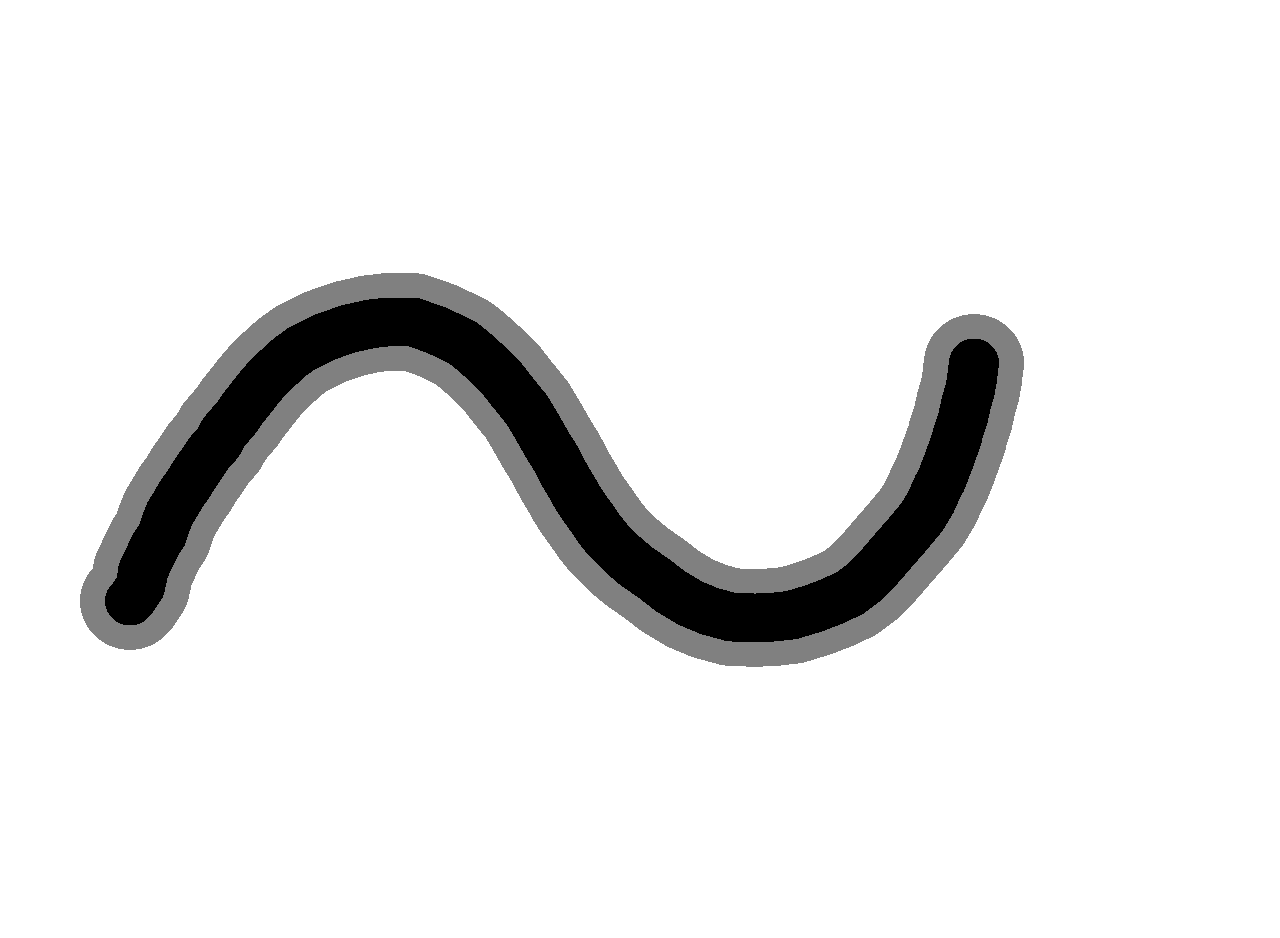
\includegraphics[width=\w]{images/stroke_triangulation/softrendered}
        
        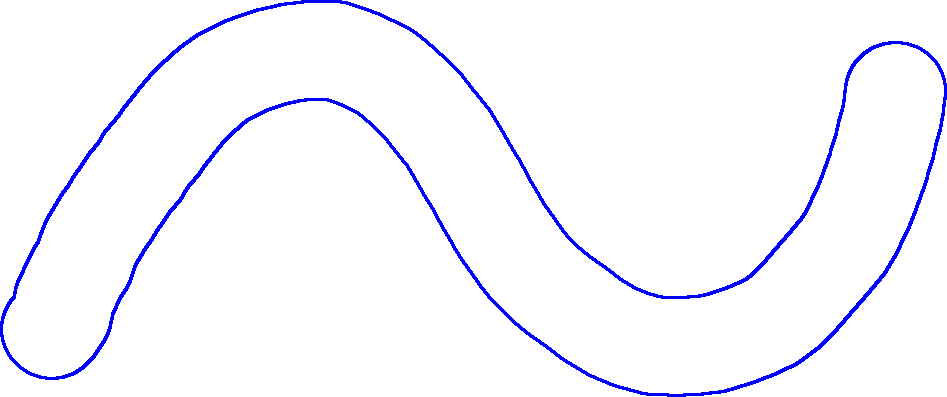
\includegraphics[width=\w]{images/stroke_triangulation/hardpruned}
        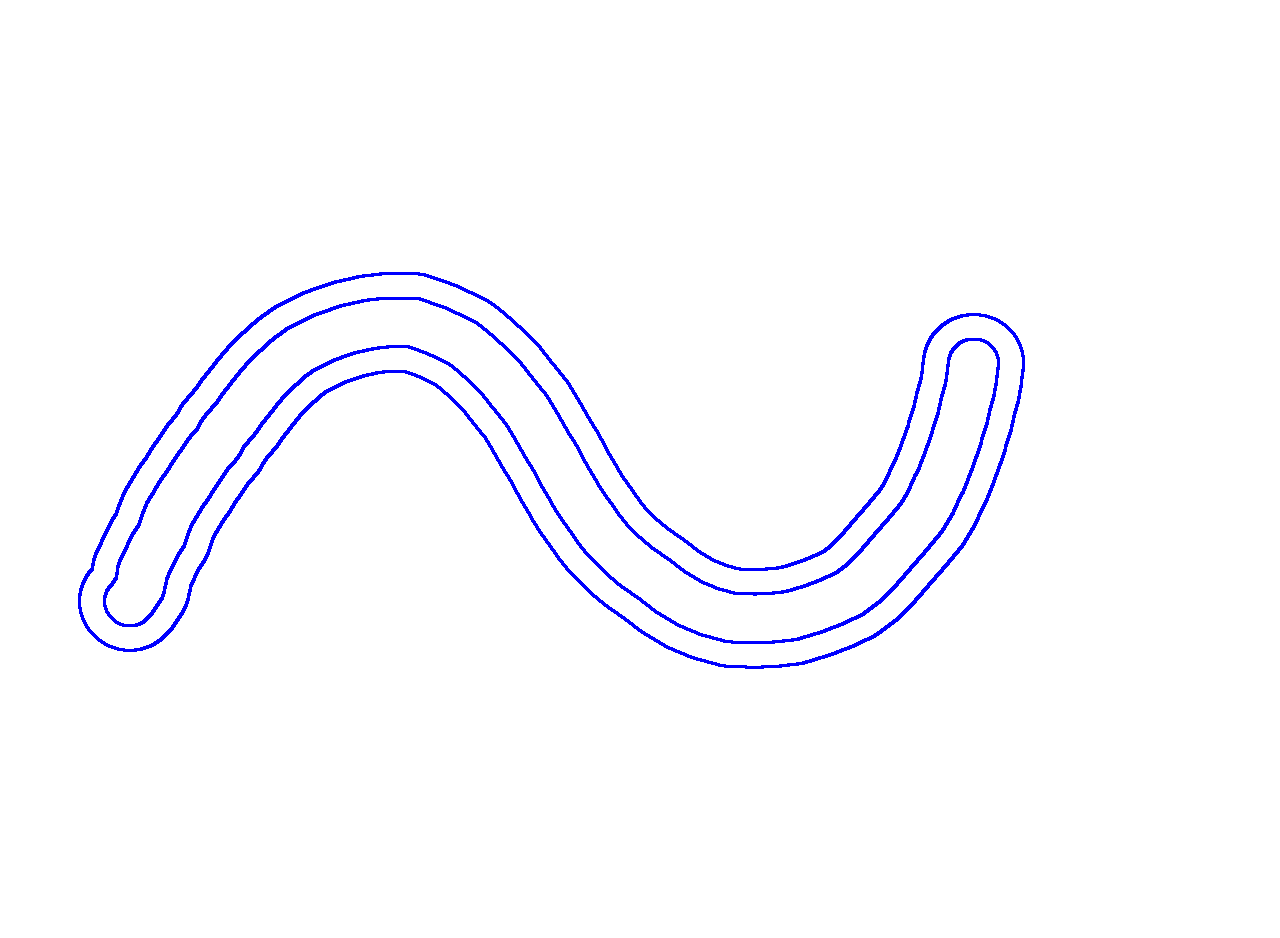
\includegraphics[width=\w]{images/stroke_triangulation/softpruned}
        
        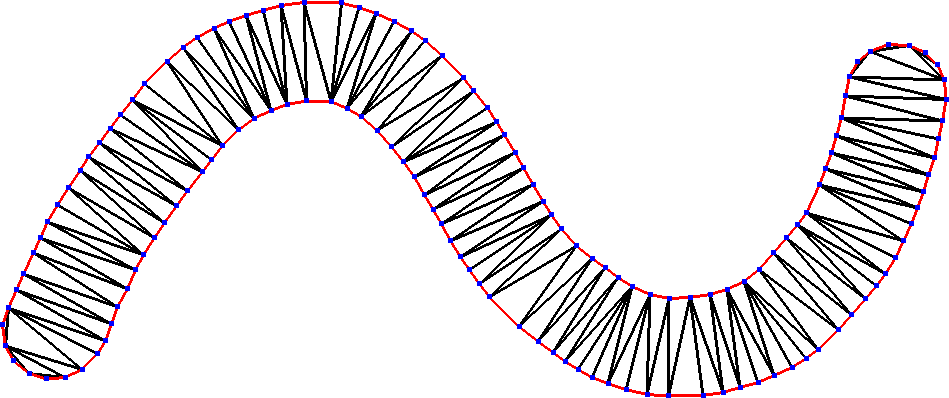
\includegraphics[width=\w]{images/stroke_triangulation/hardmesh}
        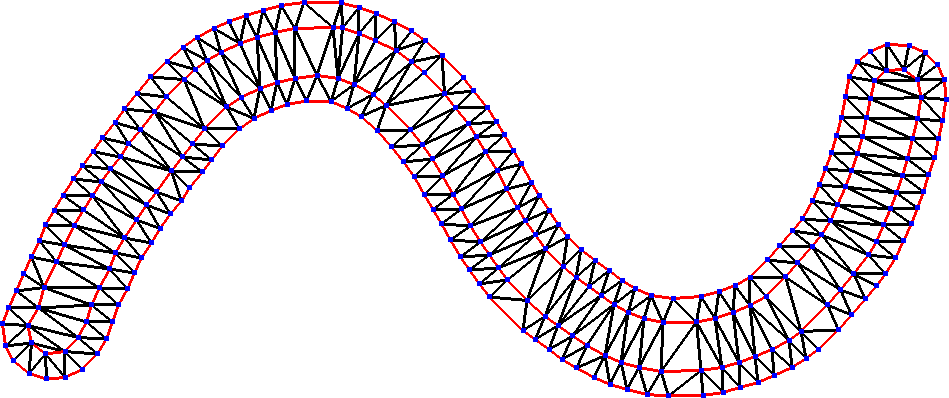
\includegraphics[width=\w]{images/stroke_triangulation/softmesh}
    \caption{Left: A hard stroke is rasterized, the contour is found, and a triangle mesh is generated.
             Right: A soft stroke is rasterized in two different shades of gray, two contours are found,
             a triangle mesh is generated with a boundary separating the inner and outer parts of the stroke.}
    \label{fig:rastertotriangles}
\end{figure}


% 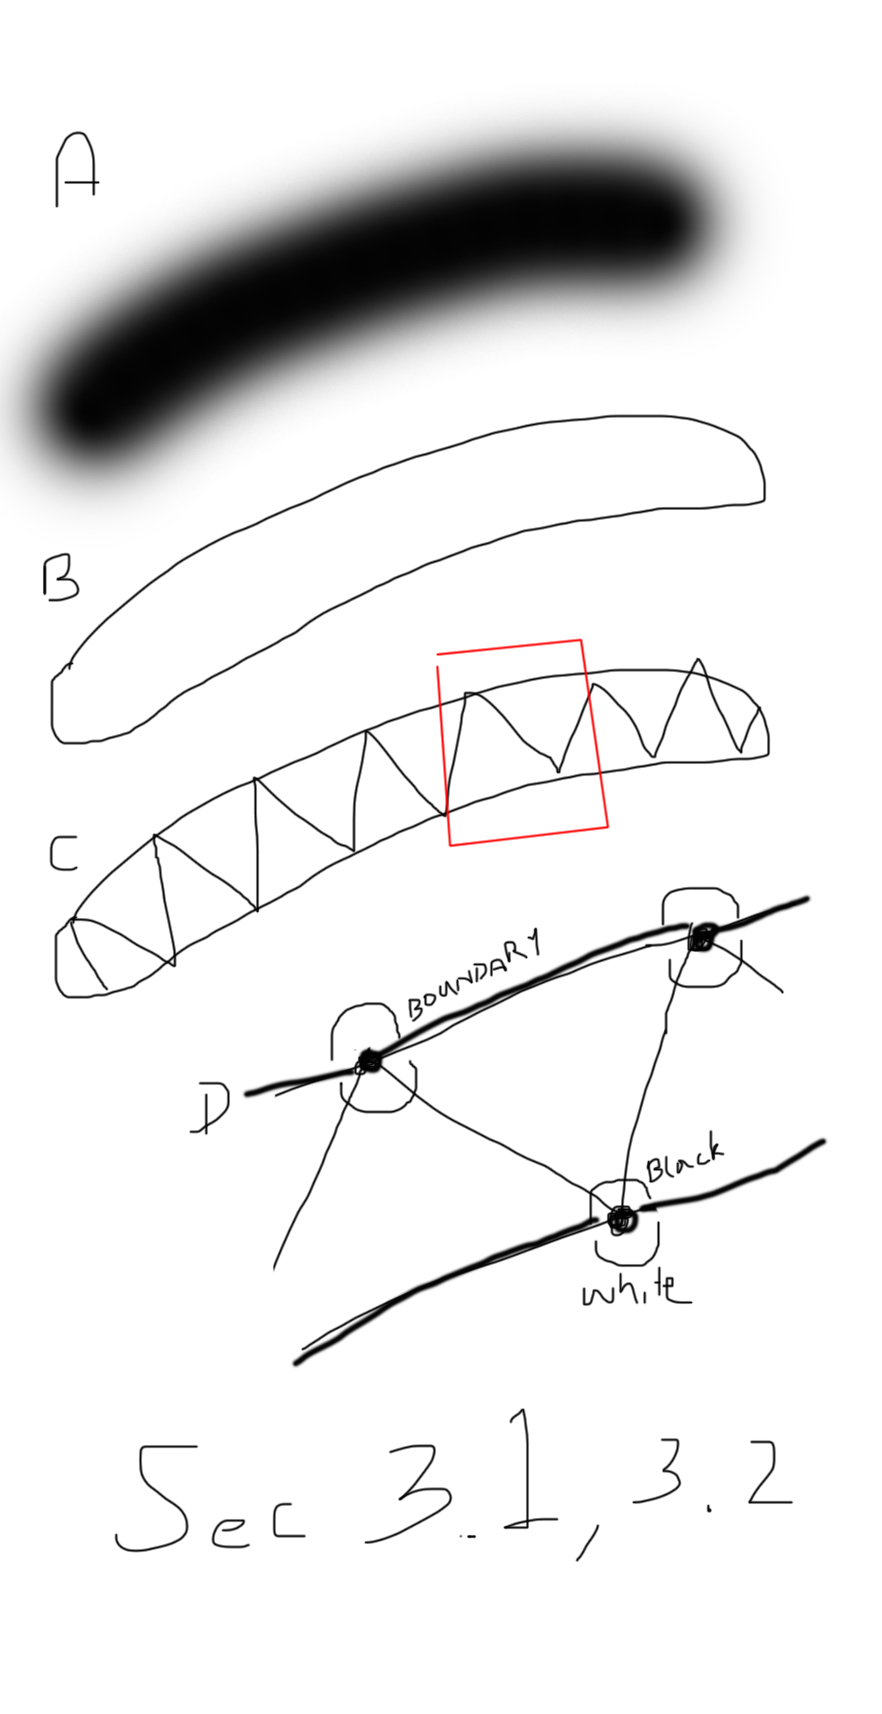
\includegraphics[height=1.5in]{images/triangulationprocess}

\subsection{Soft Strokes}
The above procedure converts a hard brush stroke into a triangle mesh. A more challenging
case is converting a soft brush stroke with linear gradient into a triangle mesh. A soft stroke has two
components, an inner hard stroke and an outer gradient stroke. Since the triangles in the inner and
outer parts of the stroke must be colored differently, none of the triangles may cross the boundary
between the hard and soft regions.

This representation needs a slightly different procedure. The user's mouse motion
is captured in two sets of polygons. The first set describes the outer soft stroke and the second set describes
the inner hard stroke. Next the outer stroke polygons are rendered in 50\% gray and the inner stroke
is rendered in black. This means the boundary of the outer stroke is the 25\% gray iso-contour and the
boundary of the inner stroke is the 75\% gray iso-contour.

Again, using marching squares these contours are extracted and then pruned. The boundaries and points
derived from the contours are given to Triangle and a mesh is returned. This mesh represents the soft
stroke where no triangle crosses the boundary between the soft and hard regions
of the stroke. Points on the contour of the inner stroke will have color arcs with the stroke color,
while the points on the contour of the outer stroke will have transparent color arcs. This gives
all triangles connecting the inner and outer strokes a linear gradient (again see Figure~\ref{fig:softarcs}).
Figure~\ref{fig:rastertotriangles} shows the process of triangulating both hard and soft strokes.

% \begin{figure}
%     \centering
%         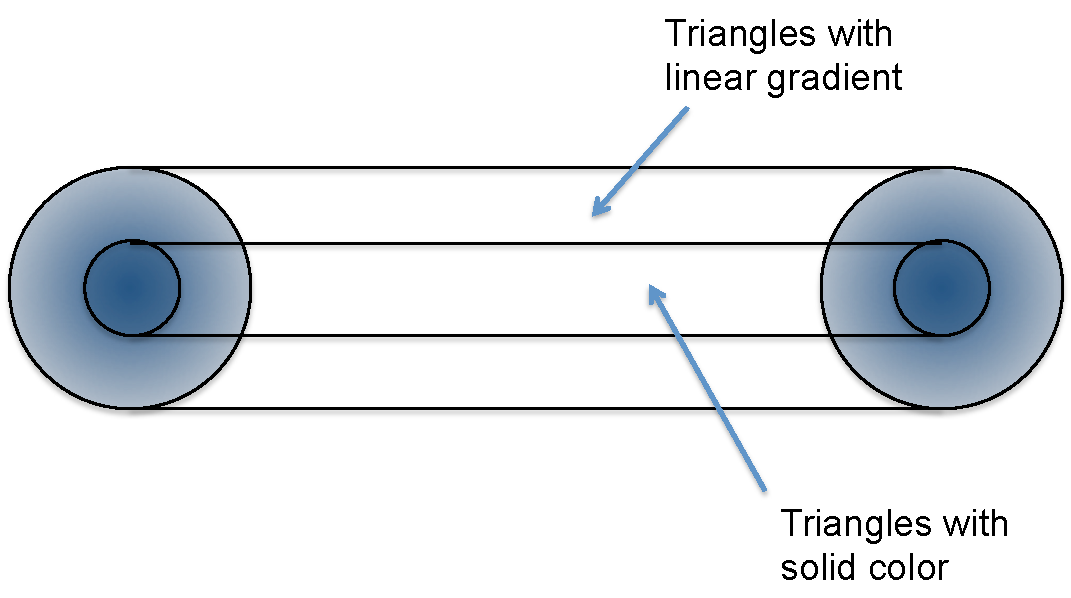
\includegraphics[height=1.5in]{images/softstroke}
%         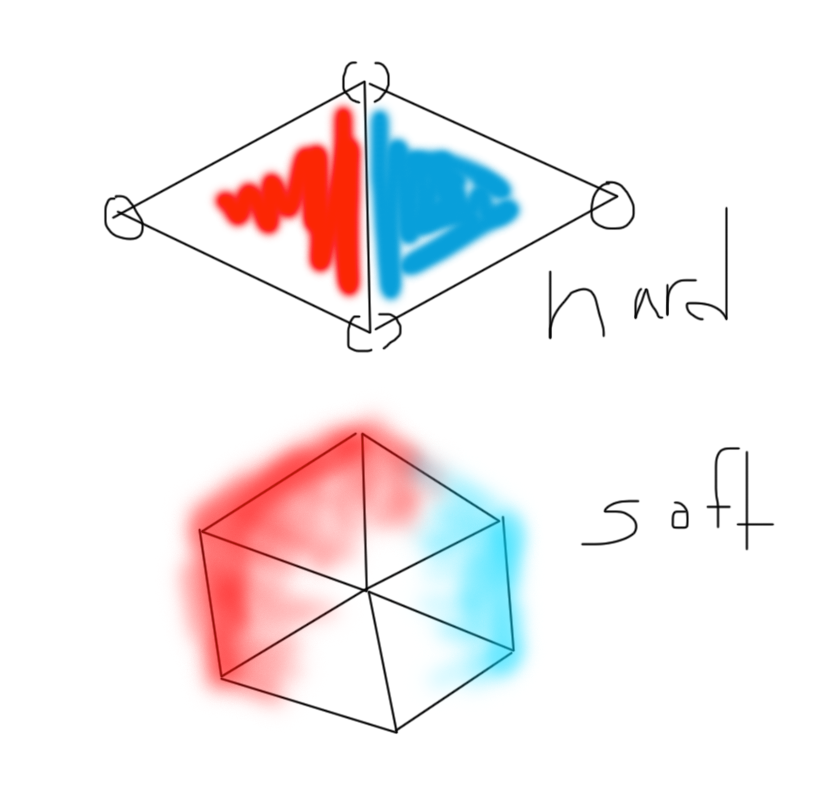
\includegraphics[height=1.5in]{images/hardvssoft}
%     \caption{Place Holder.}
% \end{figure}

\section{Compositing Strokes}
Once the stroke has been converted to triangles by the above procedure it is necessary to
composite the stroke onto the canvas. This is accomplished in two steps. First, the points
and boundaries from the triangulation of the stroke are added to the canvas and a new
triangulation is found. Second, the color arcs for the old and new points are updated.
We also discuss the challenge intersecting boundaries pose for the algorithm, as well
as a technique to reduce the number of triangles that are retriangulated on the canvas.


\subsection{Adding Points to the Canvas}

Every canvas begins with an initial set of points distributed along the edges. These
points have boundaries connecting them. These points are originally part of a number of triangles which
divide the canvas.

In the simplest approach, the points and boundaries from the new stroke are added
to the list of points and boundaries already stored on the canvas. All of this data is given to Triangle
to produce a new mesh (see figure~\ref{fig:firststrokes}). The new mesh contains all of the points of the old and new strokes. Since
all of the boundaries are stored and given to Triangle, the stroke edges are preserved. This means that
no triangle can cross the boundary of a stroke. Without this constraint, it would be impossible to correctly color the
triangles since they would straddle color arcs. Once a new mesh is formed the color arcs of the 
new and old points must be computed.


\begin{figure}
    \centering
        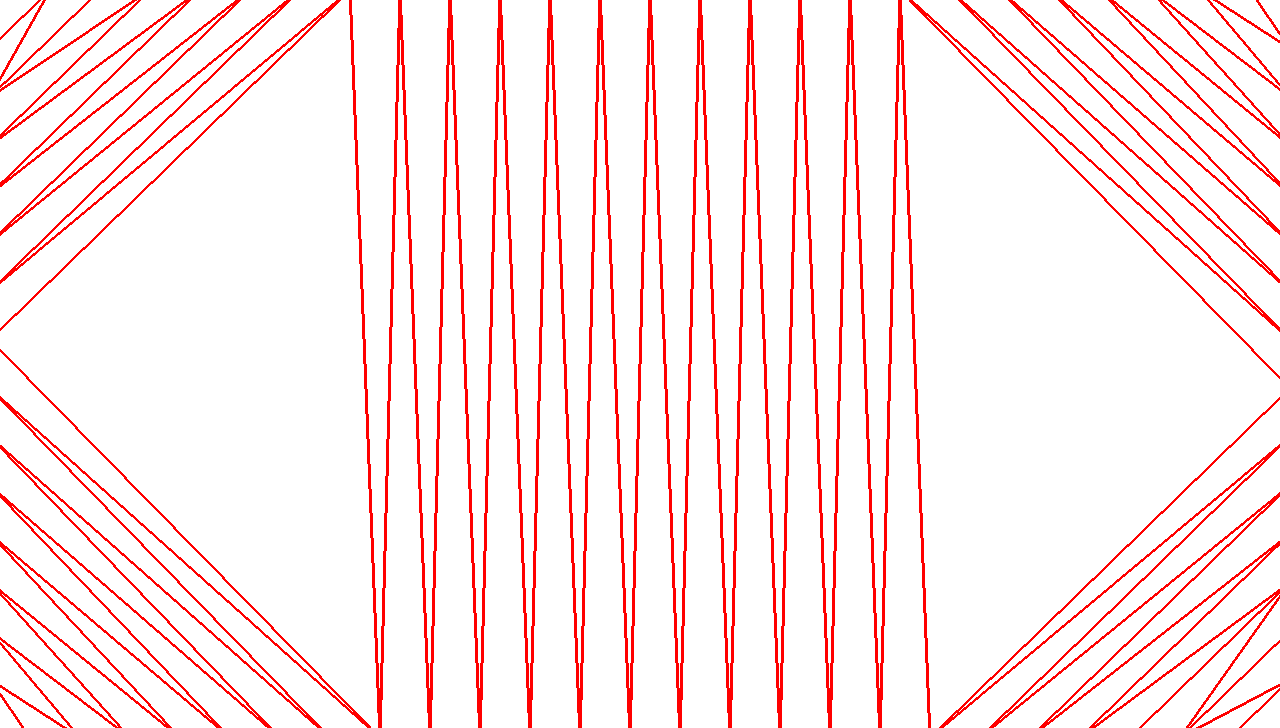
\includegraphics[width=.23\textwidth]{images/emptycanvas}
        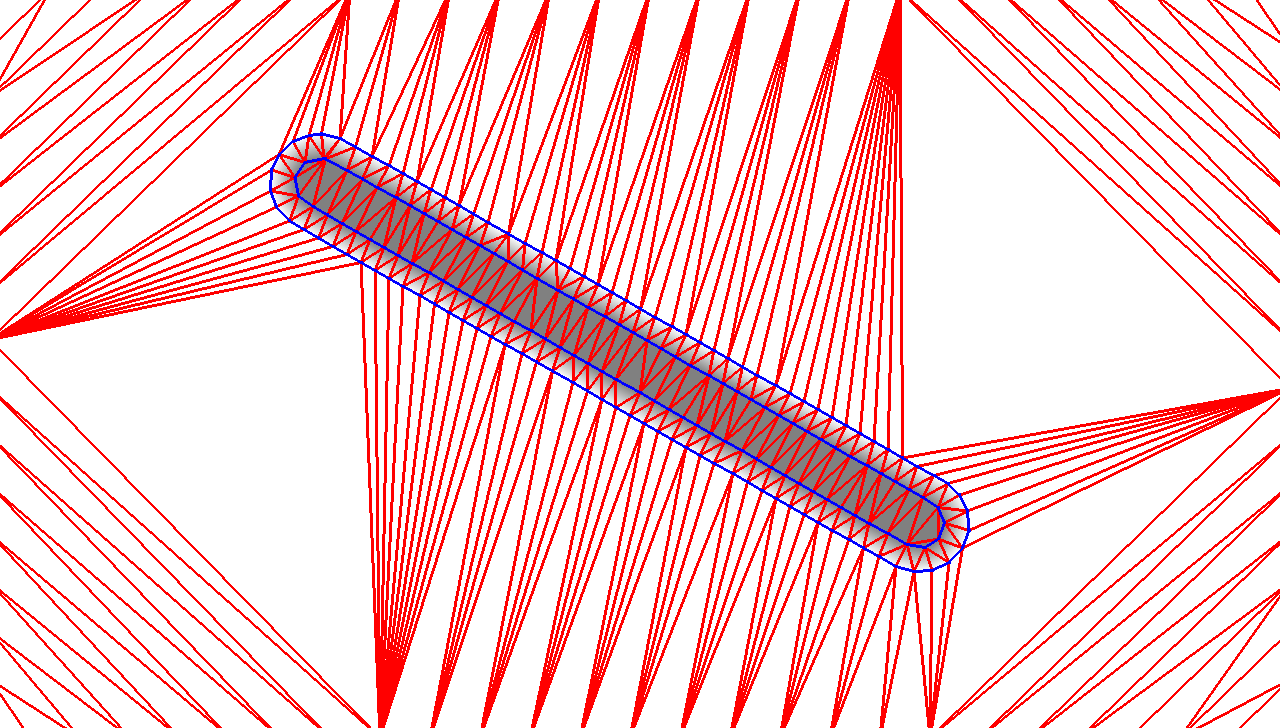
\includegraphics[width=.23\textwidth]{images/canvaswithonestroke}
    \caption{The figure on the left shows an empty canvas with a number of points and boundaries defined along the edges
             to provide the initial triangulation. The figure on the right shows how a stroke is composited onto
             the empty canvas. Blue edges are boundary edges. Red edges form the triangle mesh with the blue edges.}
    \label{fig:firststrokes}
\end{figure}


\subsection{Determining Colors}
All color compositing is done with regular RGB alpha blending.  The color arcs for new points depend on two values, the color of the stroke and the color
of the canvas at that point. The points on a hard stroke will have two color arcs. One
arc describes the inside of the stroke. The color for this arc is the color of the stroke
composited over the color of the canvas at that point. The other arc describes the outside
of the stroke. The color for this arc is just the color of the canvas at that point. The
points on a soft stroke will each have one color arc. The color arc for points on the inner
contour is the color of the stroke composited over the color of the canvas at that point.
The color arc for points on the outer contour is the color of canvas at that point (because the outer edge of the soft stroke is completely transparent).
This gives any triangle connecting inside and outside contour points a linear gradient
from the stroke color composited over the canvas color to the canvas color.

The color arcs for old points remain the same unless part of the new stroke covers it.
In this case the colors in each arc must be replaced with the stroke color composited over
the old color of the arc. If the new stroke is soft then the color at the location of
the old point must be determined through bilinear interpolation before compositing.



\begin{figure}
    \centering
        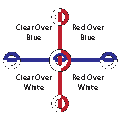
\includegraphics[width=.2\textwidth]{images/intersectioncolorarcs1final}
        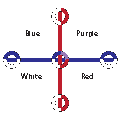
\includegraphics[width=.2\textwidth]{images/intersectioncolorarcs2final}
        
    \caption{Left: A red stroke is composited over a blue stroke. An intersection
            point is inserted in the center and four color arcs must be determined. Right:
            The four colors are resolved as the four combinations of the red stroke's color
            arcs composited over the blue stroke's color arcs.}
    \label{fig:intersectioncolors}
\end{figure}

\begin{figure*}
    \centering
        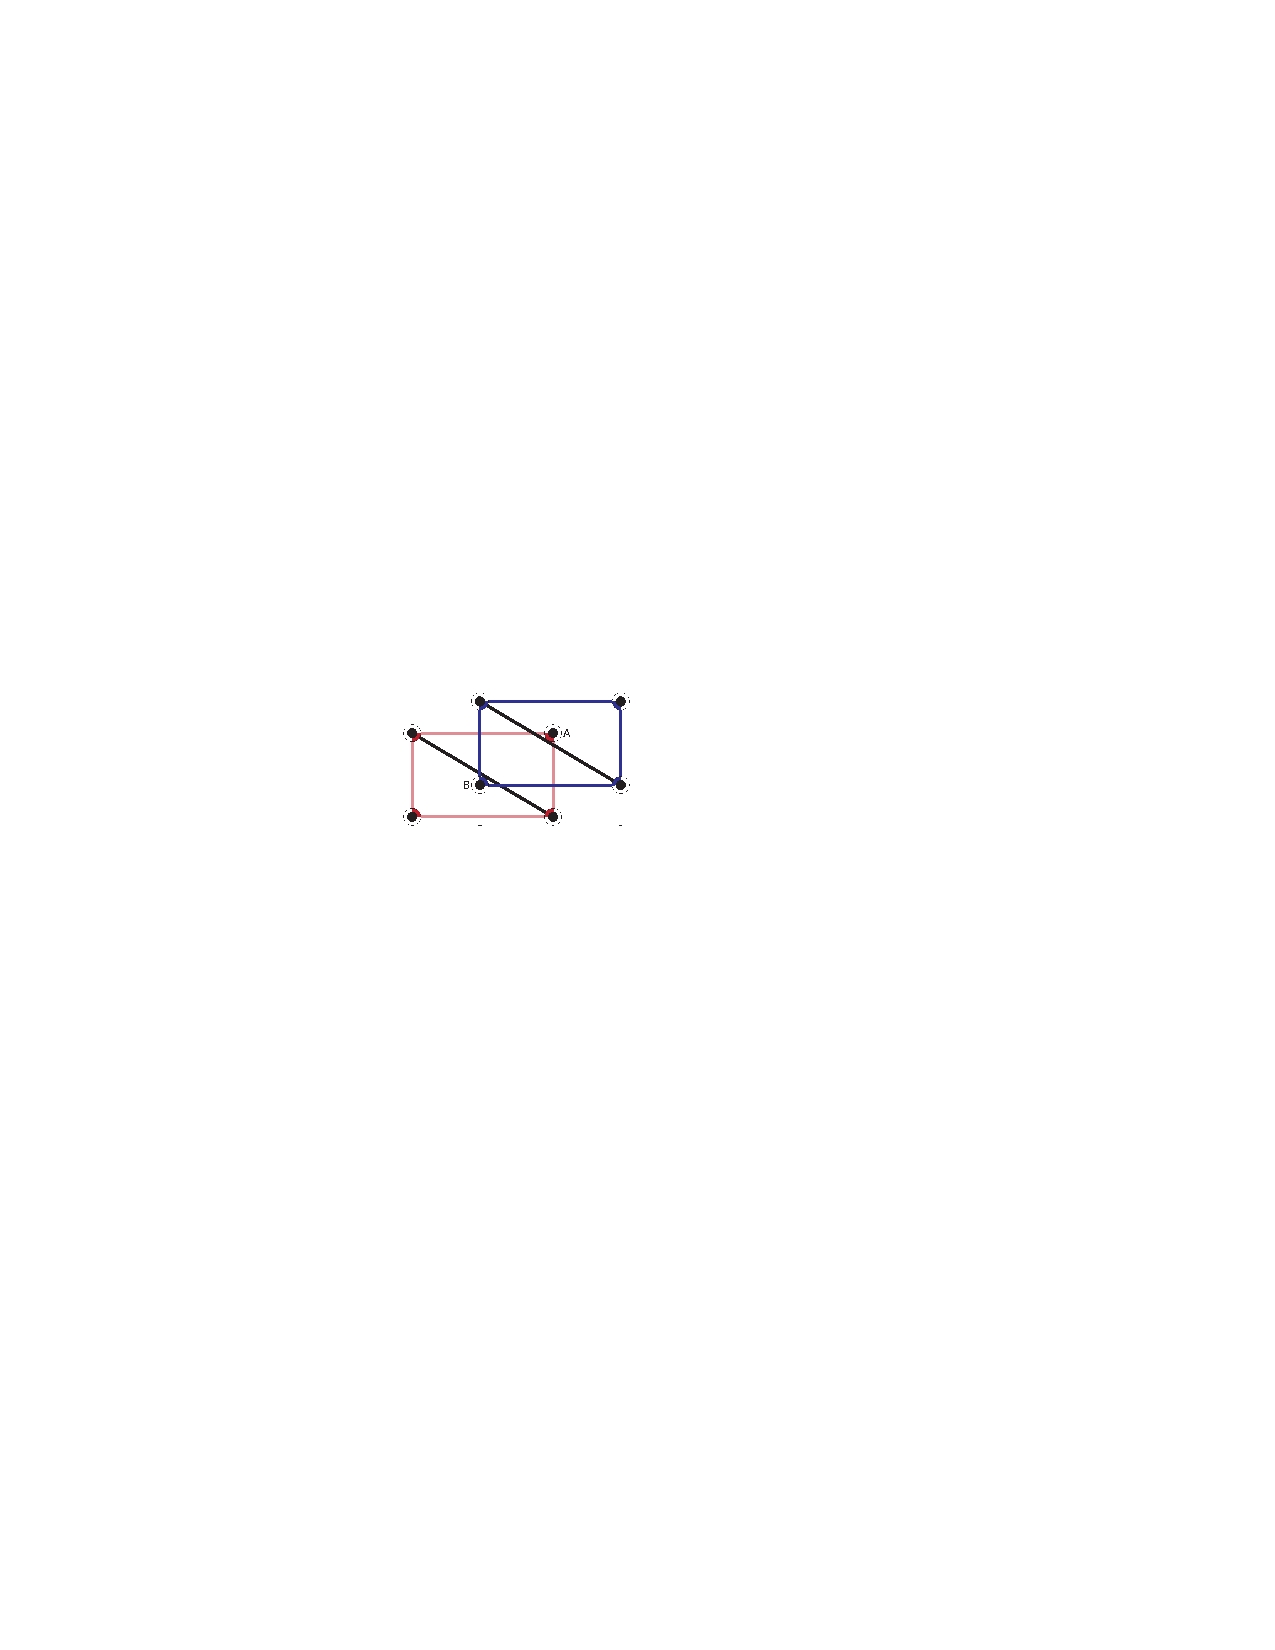
\includegraphics[width=.32\textwidth]{images/composite21}
        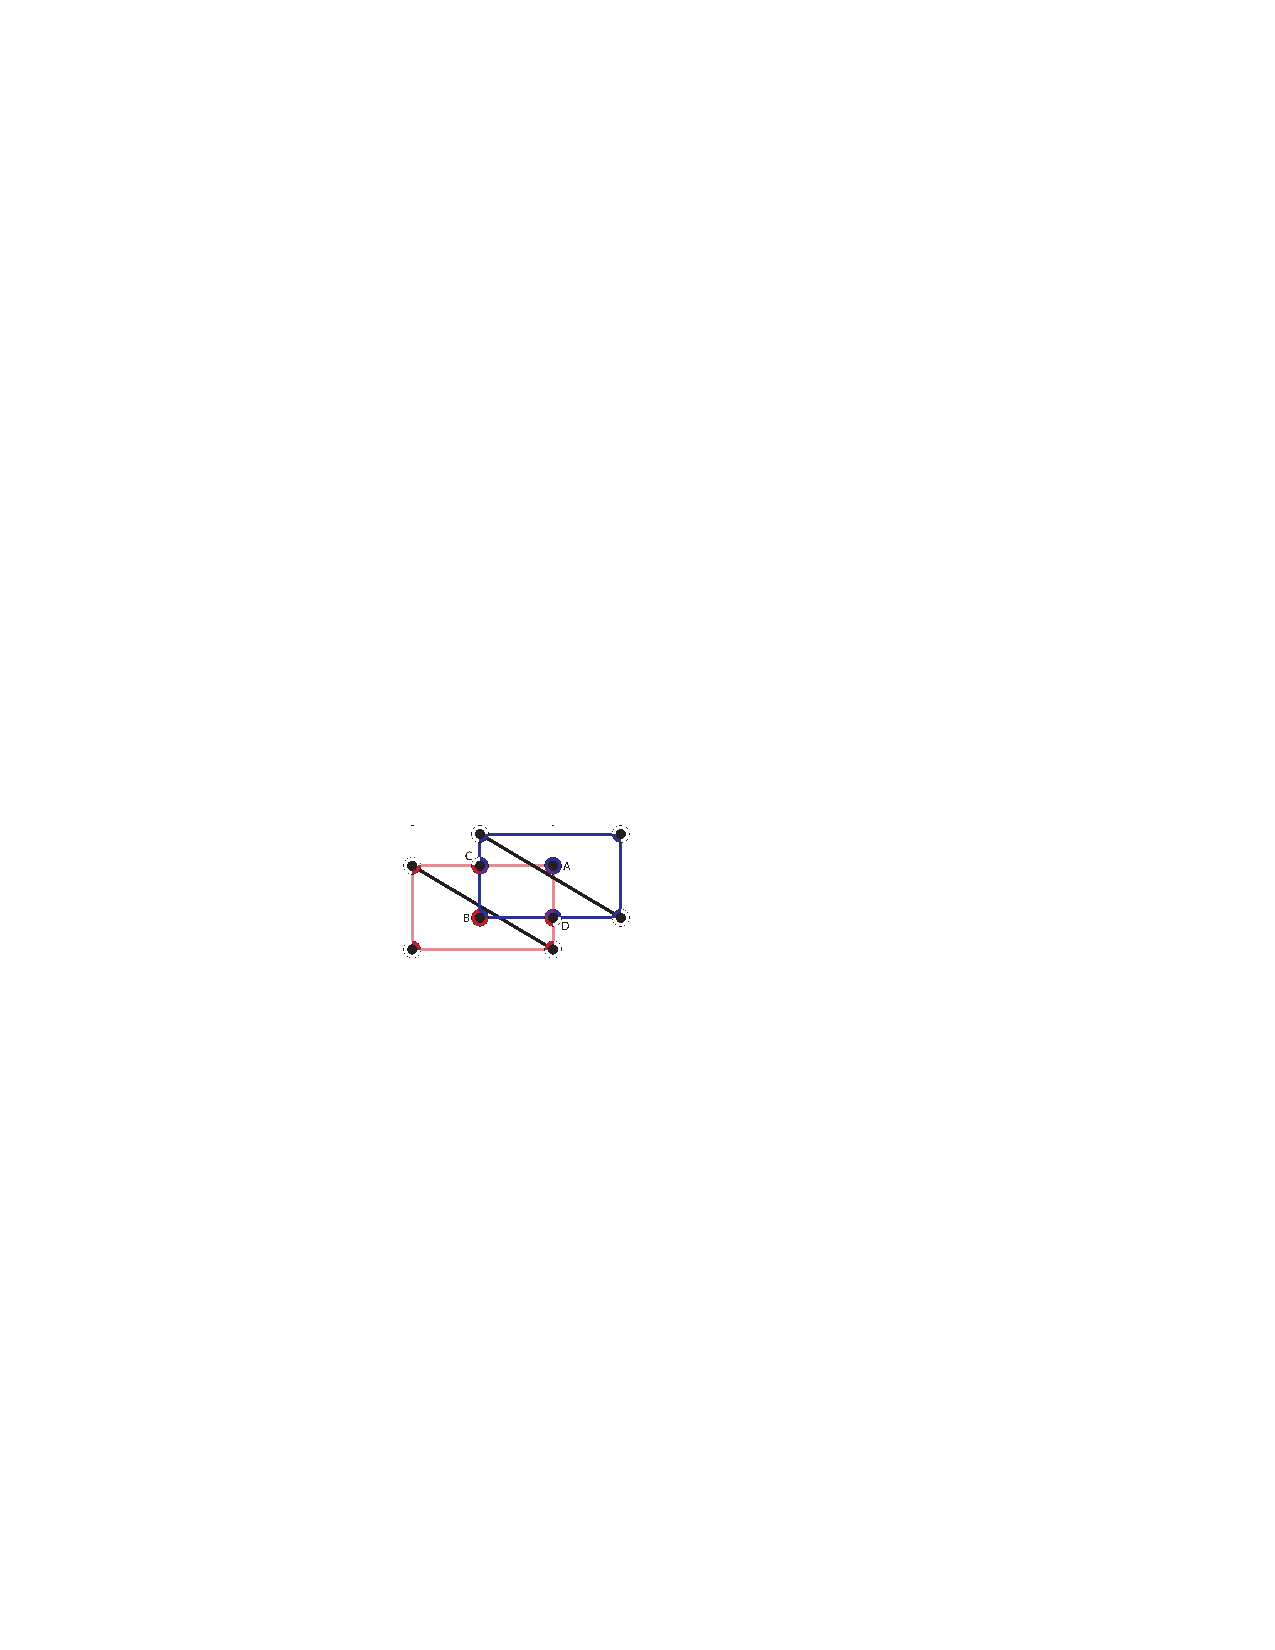
\includegraphics[width=.32\textwidth]{images/composite22}
        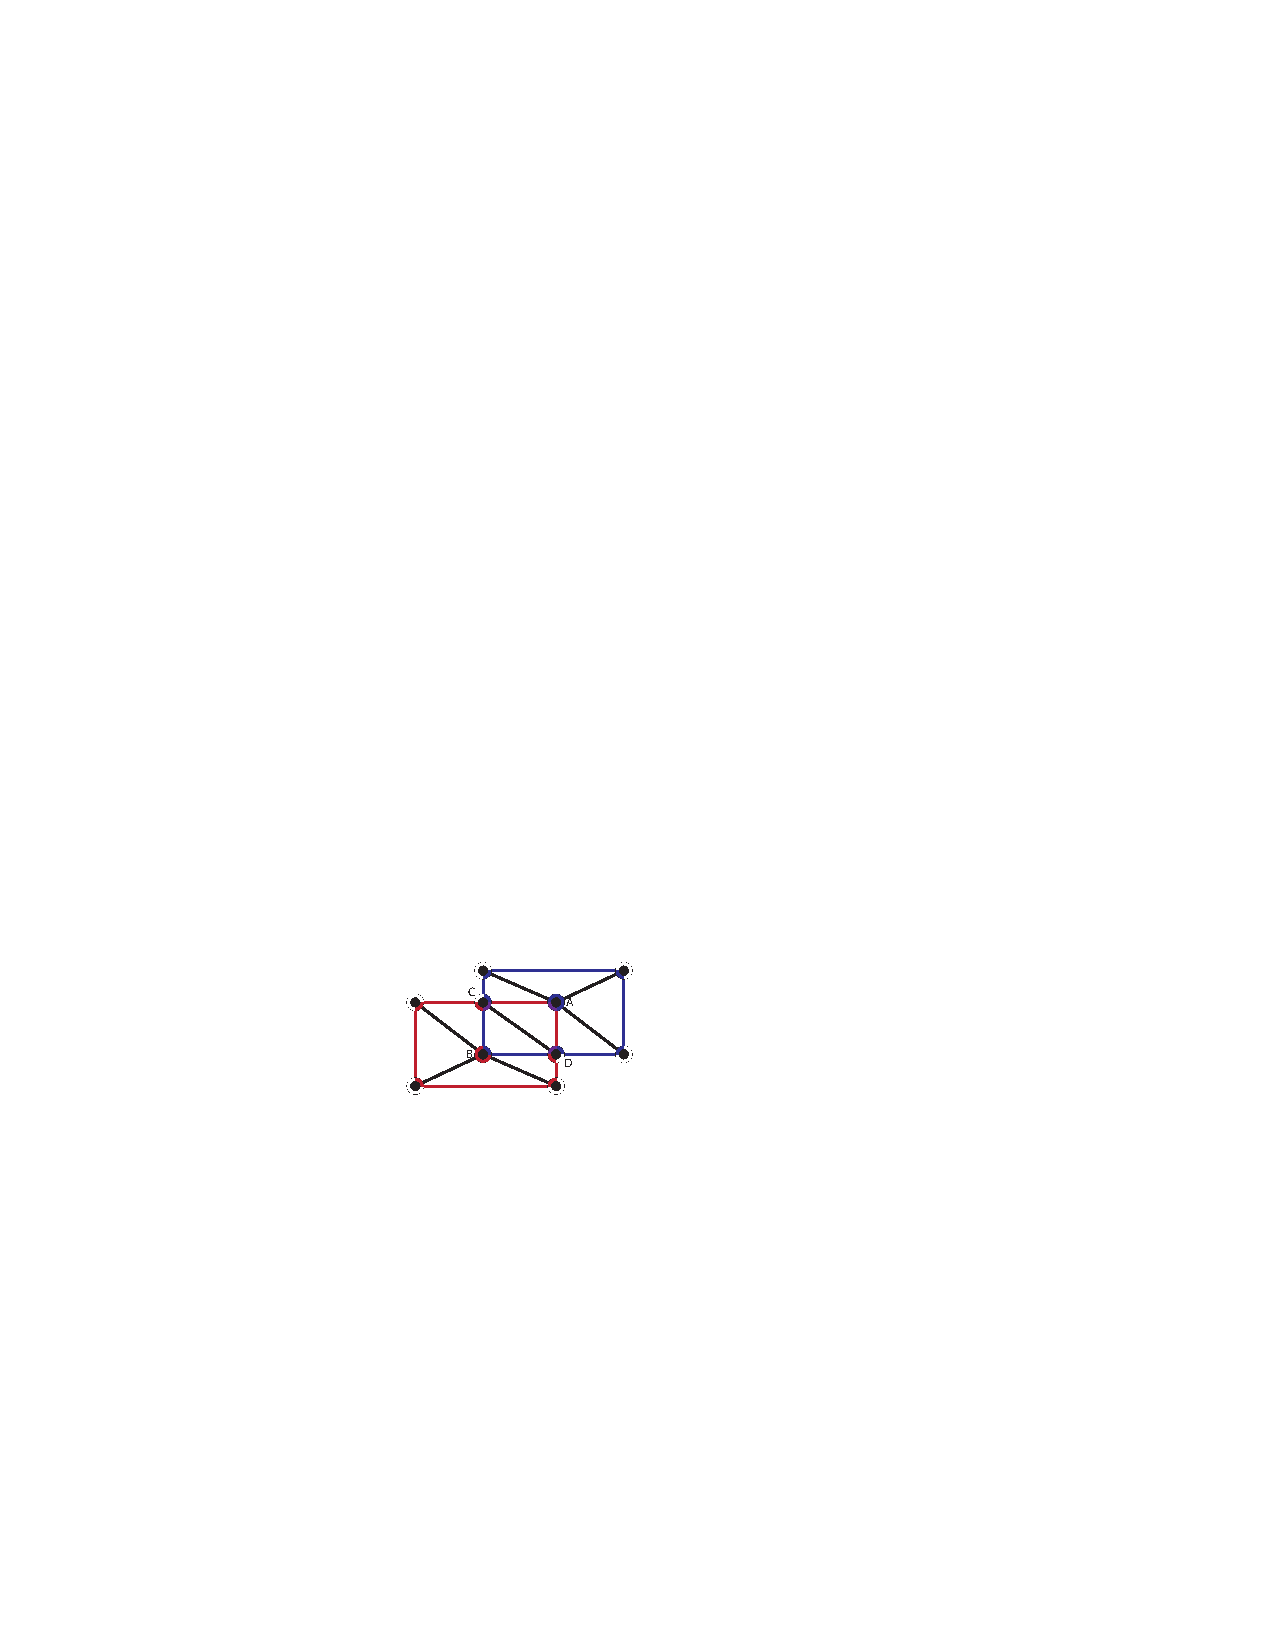
\includegraphics[width=.32\textwidth]{images/composite23}
    \caption{Left: A blue stroke is composited over a red stroke. Point A is covered
             by the the blue stroke and point B is on top of the red stroke. Middle:
             New color arcs are determined. Both of A's color arcs are composited
             with the blue stroke which turns red to purple and transparent to blue. Similarly
             both of B's color arcs are composited on top of the red stroke which turns
             blue to purple and transparent to red. Two intersection points C and D are
             added. Their color arcs are determined by examining neighboring points. Right: 
             A new triangle mesh is generated to preserve boundaries. Note that triangles
             in the intersection will be purple.}
    \label{fig:colorarcdeterminer}
\end{figure*}

\subsection{Intersection Points}

When Triangle is asked to triangulate a set of points with intersecting boundary edges, it must
insert a point at the intersection, since without it at least one triangle would have to
cross a boundary. These points are introduced with no color information, but the final colors for 
all of the other points in the mesh have already been determined.

An intersection point lies on two boundaries and therefore has four boundary edges emanating from it. 
To determine the colors of an intersection points requires knowing the colors associated with
other points on the boundaries. For both boundaries, travel both directions to the first point with color data. Note this may not
be the first point on each side since this intersection point may be adjacent to other intersection
points also without color data. For both boundaries, the colors in the color arcs are linearly interpolated. 
This yields four average colors, two from the new stroke boundary and two from the old stroke boundary.
The colors from the new stroke are composited over the colors from the old stroke to yield four new
colors, one for each region defined by the boundary intersections (see figure~\ref{fig:intersectioncolors}) 

An example of how color arcs are determined for both intersection and regular points see figure~\ref{fig:colorarcdeterminer}.

\subsection{Finding Modified Points}
The above procedure has two important drawbacks. First, it processes many points that do not need
consideration which takes a considerable amount of processing time. Second, since it acts on the whole
canvas, local changes can have global effects. To avoid this problem the algorithm determines
which triangles can remain
and which triangles need to be included in the re-triangulation (see Figure~\ref{fig:modified}). To accomplish this a static grid
is generated and all of the cells which contain a triangle from the new stroke are marked. 
The set of triangles from the old triangulation that intersect these grid squares are found.
The set of edges from these triangles that do not intersect these grid cells form a ring
around the area of our new triangles. The edges in this ring become constraints
in the triangulation. All of the points and constraint edges from the old triangulation are
included as well as the points and constraint edges from the new triangulation. Triangulating
these points and edges gives the new geometry for the modified area and has no effect on any
other part of the canvas. Therefore, the old triangles from the rest of the canvas can be reused. 
The new triangulation combined with the old triangles give a new triangle mesh representation of the entire canvas.



\section{Discussion and Results}
Paintings made with the system can be seen in Figures~\ref{fig:face}, \ref{fig:teaser}, \ref{fig:stop} and \ref{fig:boxes}.  Here we first consider how the complexity of the algorithm grows both in time and geometry.
The results from this analysis and our experience with the system have lead to a number of observations.

\subsection{Complexity}
To find the growth rates of the algorithm we performed two experiments. 
First, the program drew fifty random strokes without zooming.
Next, the program drew fifty random strokes with random zoom level for each stroke.
Geometry grows fastest when many strokes are composited on one another. When not zooming, strokes
must cover the same area of canvas over and over. This
results in more geometry and therefore takes longer to render. The zooming case explores different
areas of the canvas and therefore results in less overlapping geometry. This situation should result
in less complex geometry and therefore take less time.

Figure~\ref{fig:numtriangles} shows the zooming case grows linearly while the non-zooming case
appears to grow quadratically. This is expected since every new stroke has the chance to overlap
all of the old strokes. Therefore each new stroke does not just add a constant amount of geometry, but 
due to intersections with previous strokes extra intersection points are added. This results in a linear
increase in the amount of geometry per stroke yielding a quadratic growth rate. However, in the zooming case each stroke rarely overlaps and therefore
intersection points are rarely added. In this case the geometry increases by a constant amount per stroke which yields
a linear growth rate.

Figure~\ref{fig:timing} gives a similar result for the cumulative time strokes take to render. Both
the zooming and non-zooming cases grow non-linearly over time. However, the non-zooming case takes
longer for the reasons described. It is not unexpected that even the zooming case grows non-linearly
since even though the geometries involved are not becoming very complicated, the geometry of the entire
canvas is increasing linearly and must be considered even if the entire canvas is not re-triangulated.

This suggests that canvas simplification is of great importance.
The case that it is most likely to be helped is the non-zooming case with complex geometry. When lots of strokes
overlap there is usually extra geometry that does not add much detail to the drawing. By removing
this extra geometry the algorithm should achieve a steady growth rate.

\subsection{Stability}
While the Triangle library is impressively robust, there are still certain pathological geometries that can cause it to fail.  Specifically, long skinny triangles and vertices that are too close together seem to trigger triangulation failures.  Detecting these situations and fixing them, or even better modifying the geometry construction to avoid them, would solve this problem.  For example, identifying if a new vertex is too close to an existing one, and if so, merging them.  Another example is to subdivide long edges to reduce the incidence of skinny triangles.  The impact these solutions would have on processing time is something that needs to be explored.

\begin{figure}
    \centering
        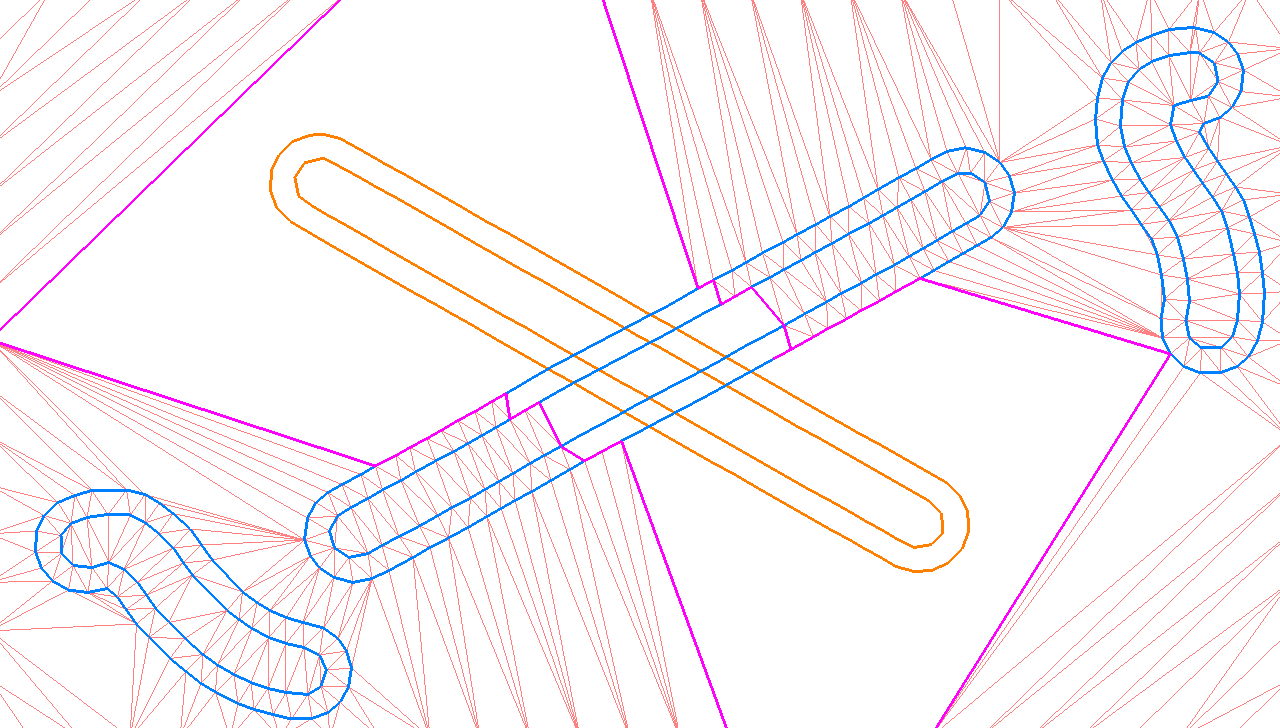
\includegraphics[width=\columnwidth]{images/grid}
    \caption{An example of how the system determines which triangles to save and which to retriangulate. Blue
    lines represent the boundaries of old strokes, orange lines are the boundaries of the new stroke, red lines are
    the triangles that will be reused, and purple lines define the area that needs to be retriangulated. The purple
    lines are edges of triangles that intersect the new stroke. Since they interesect the new stroke they are no
    longer valid and must be retriangulated. All other triangles on the canvas can be reused.}
    \label{fig:modified}
\end{figure}

\subsection{Performance}
The current implementation uses Python and PyOpenGL. Python's performance is slower than
a lower level implementation in C++ would be. The drawing of the canvas is quick with
no lag. However, the actual process to take a stroke from rasterization to triangle
representation on the canvas can be slow. On a blank canvas, strokes take less than
one second to process. However, on a canvas with lots of geometry a stroke that overlaps
that geometry can take several seconds to render. Some of this could be alleviated by a carefully optimized implementation. However, there are many calculations
necessary for the old points affected by the new stroke and the points associated with the
new stroke itself. Since these geometries can become arbitrarily complicated (in pathological cases), these
calculations can take an arbitrarily long. This brings us to the final point, simplification.

\subsection{Simplification}
No matter how good the implementation, the fact that paintings can become arbitrarily complicated as more and more strokes are added
means there must be some way to simplify the mesh. In most situations where
many strokes overlap one another, most of the geometry is redundant. For example, when an opaque stroke is laid down on top of a complex geometry, that complex
geometry no longer has any useful information since the outline of the opaque stroke
completely defines it (all vertices are the same color).  Furthermore, even with translucent or feathered strokes, a large enough number of 
composited strokes may produce complex geometry that does not add much to the visual appearance of the canvas. Some of this geometry can be reduced without noticeable changes.  To accomplish this, our proposed simplification algorithm would identify a vertex that can be removed via an edge collapse by measuring the change the collapse would cause in the image.  The change is computed as the magnitude of the color shift and the translation of a boundary.  If these deltas are below a threshold, then the collapse can proceed.  This process could be done when a stroke is added to the canvas, or continually in a background thread to avoid increasing apparent latency.  Though we have yet to implement this simplification algorithm, it is important to ensure a painter can continue to iterate on a painting without the program becoming too slow.

\begin{figure}
  \centering
  \begin{subfigure}[b]{0.5\columnwidth}
    \centering
    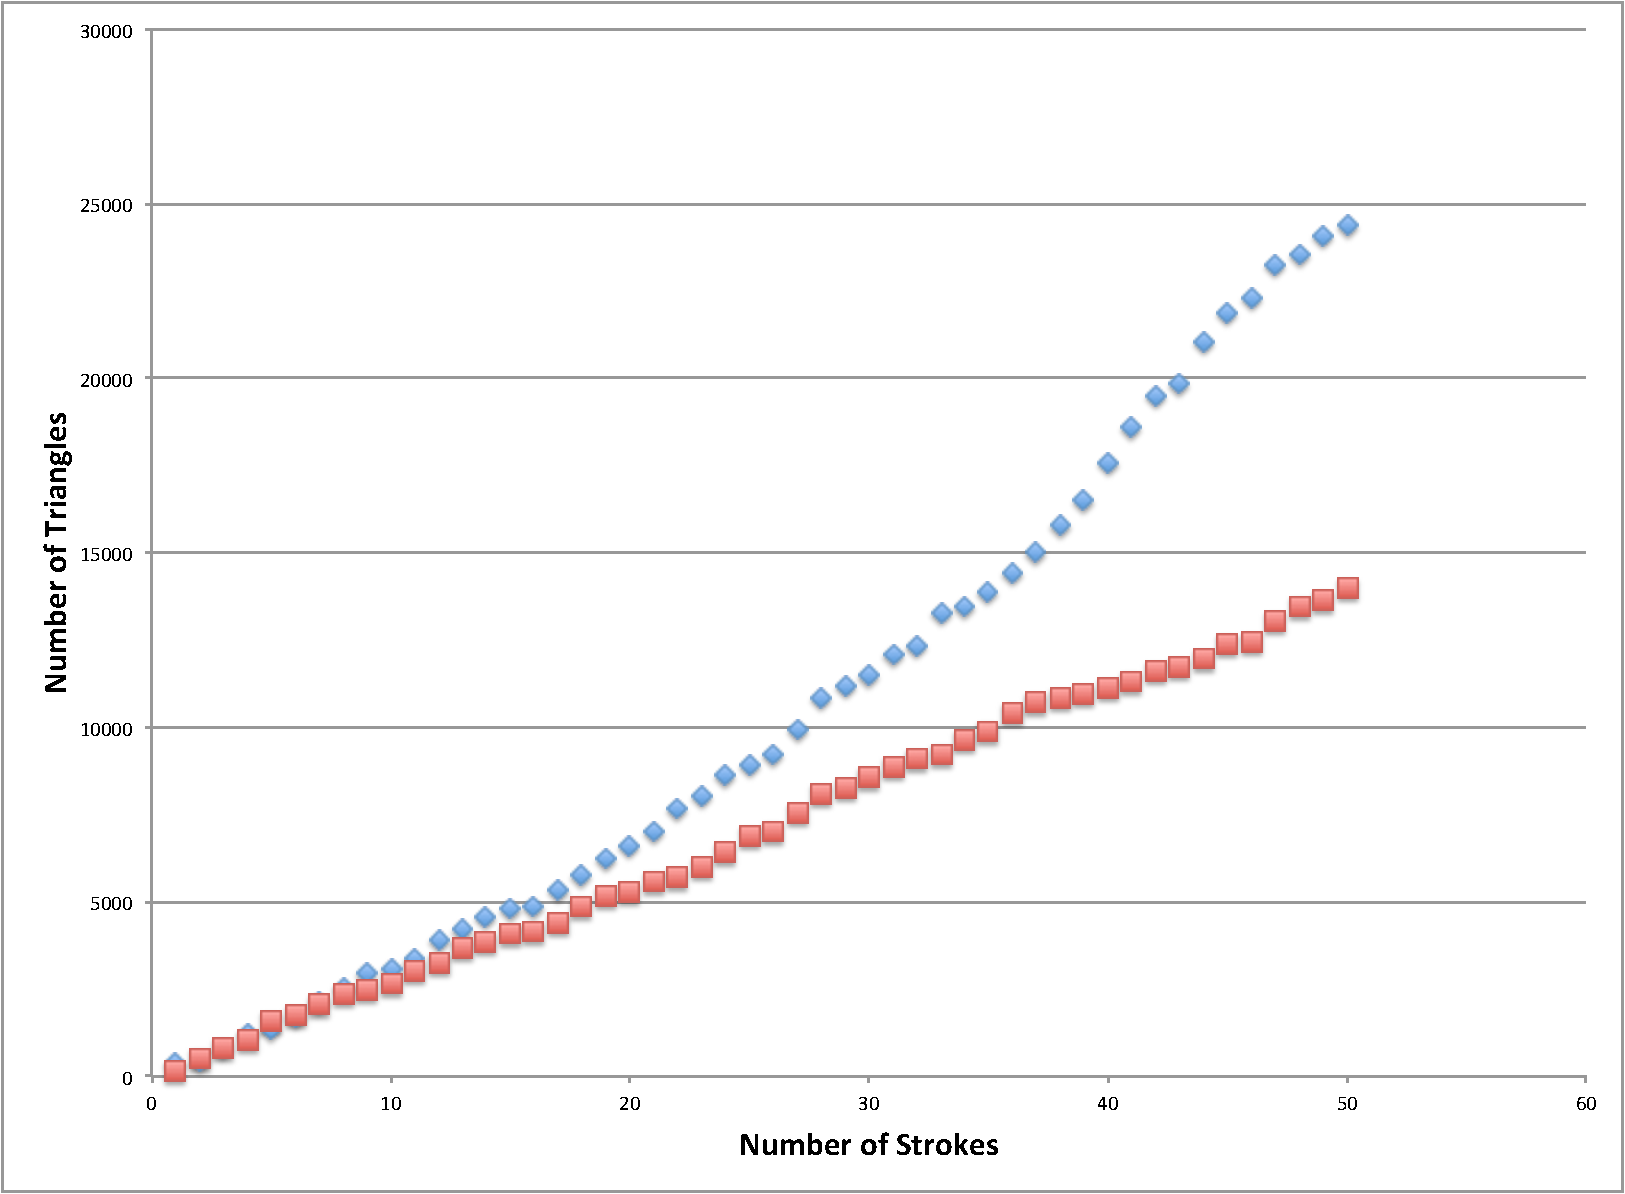
\includegraphics[width=\columnwidth]{graphs/numtriangles}
    \caption{Number of triangles}
    \label{fig:numtriangles}
  \end{subfigure}%
  \begin{subfigure}[b]{0.5\columnwidth}
    \centering
    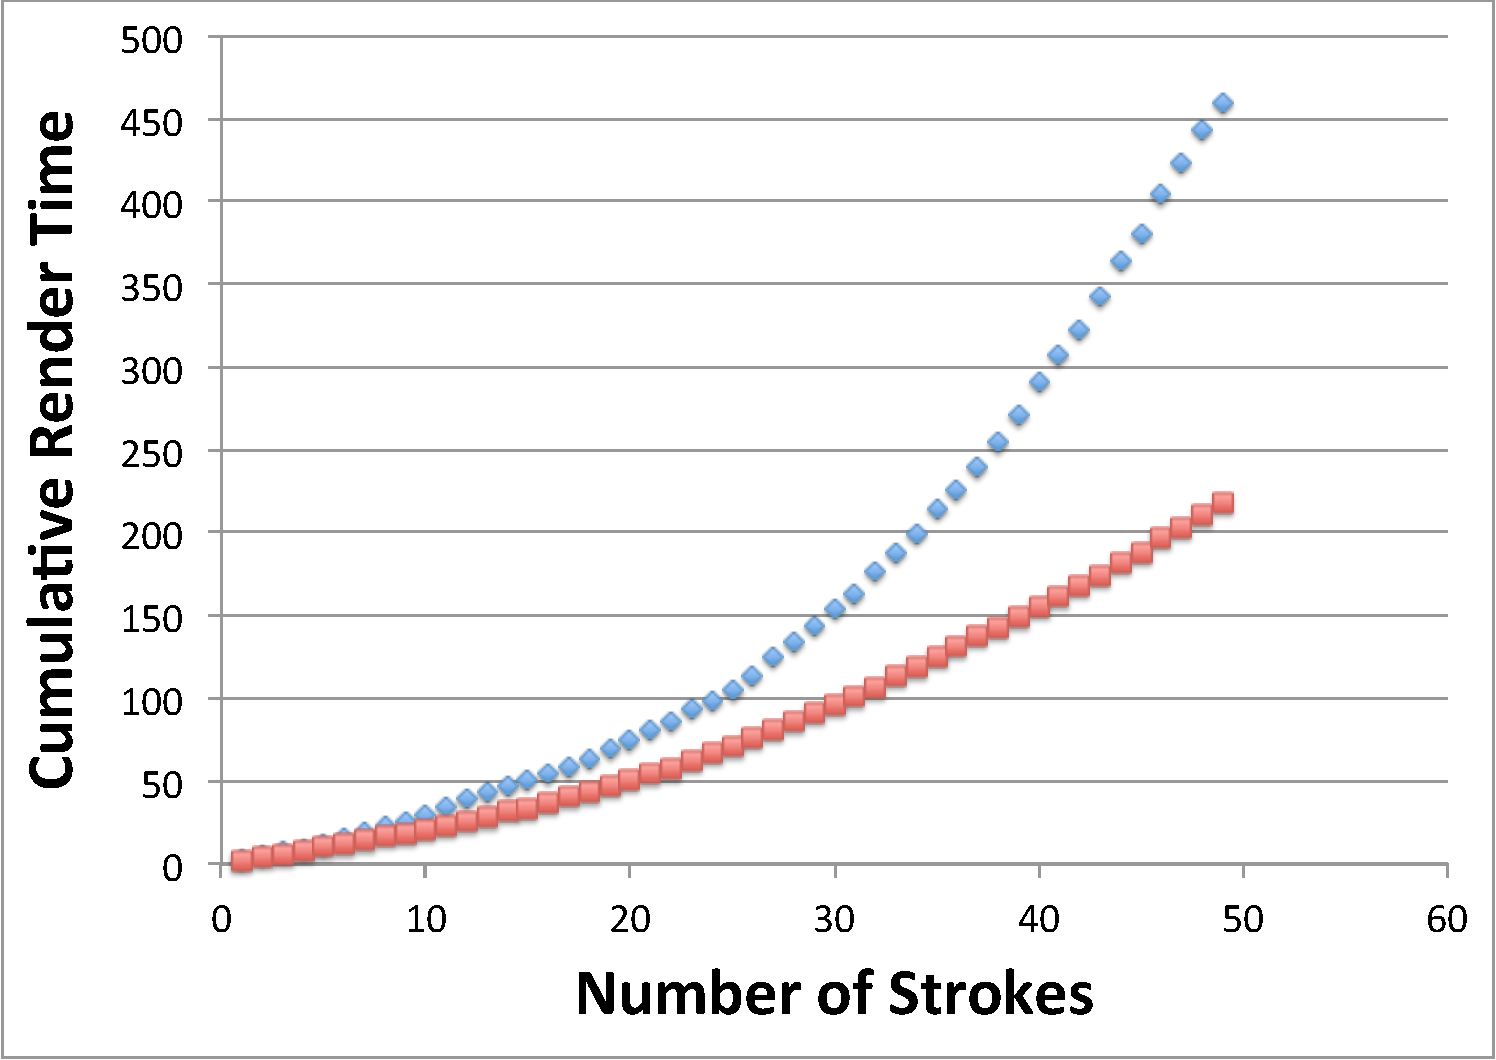
\includegraphics[width=\columnwidth]{graphs/cumulativetime}
    \caption{Rendering time}
    \label{fig:timing}
  \end{subfigure}%
  \caption{For paintings of 50 random strokes, the left graph shows the number of triangles in the canvas as of stroke $x$, and the right graph shows the cumulative render time of the painting. The blue points are the non-zooming case, while the red points are the zooming case.}
\end{figure}



% \begin{tabular}{| l | l | l | l|}
%   \hline                       
%   Number of Strokes & Triangles & Points & Boundaries \\
%   \hline                       
%   1 & 360 & 229 & 229 \\
%   2 & 506 & 302 & 310 \\
%   3 & 652 & 375 & 403 \\
%   4 & 798 & 448 & 488 \\
%   5 & 972 & 535 & 603 \\
%   6 & 1164 & 631 & 713 \\
%   \hline  
% \end{tabular}
% 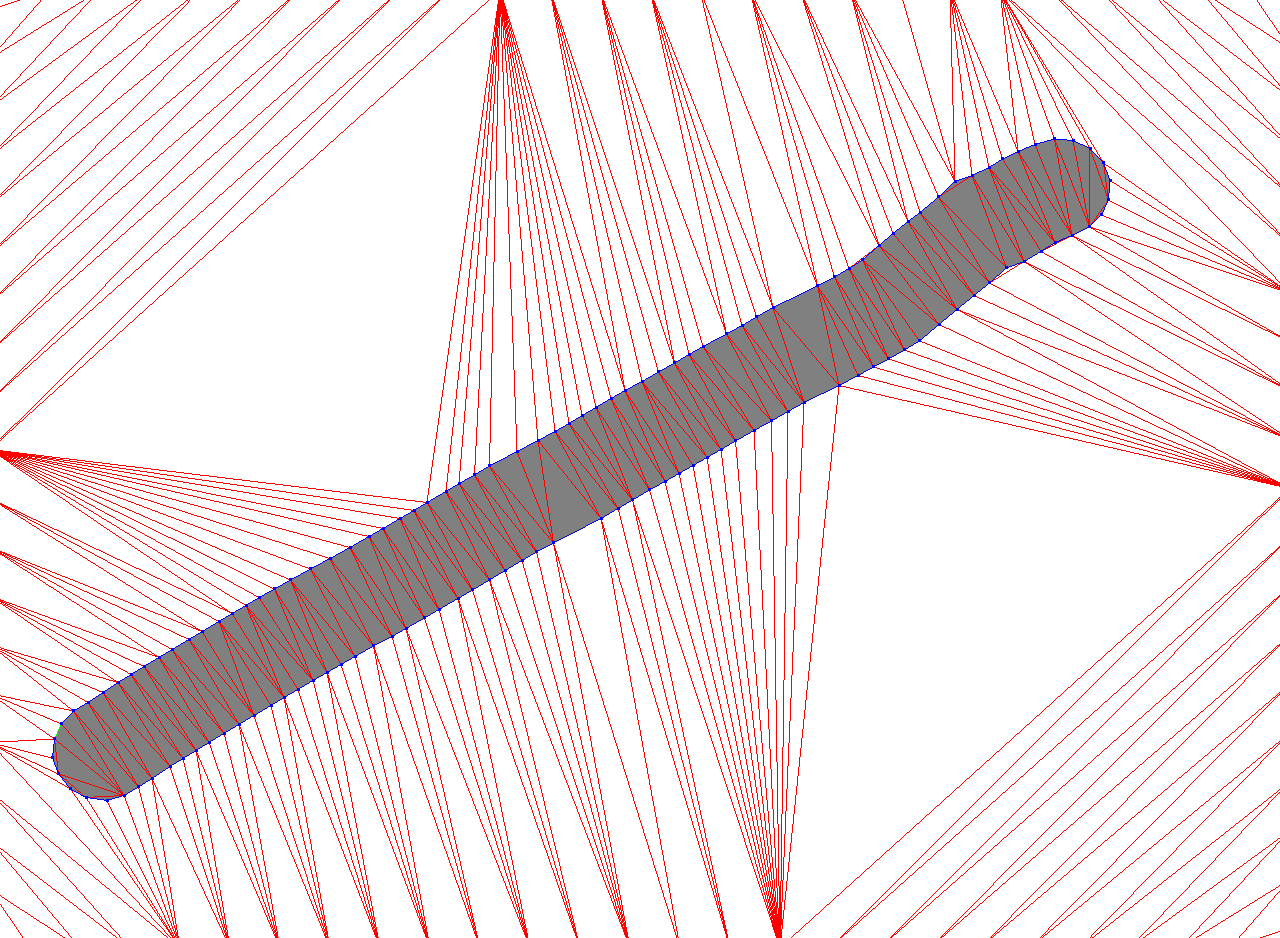
\includegraphics[height=1.5in]{images/tri360points229edges229}
% 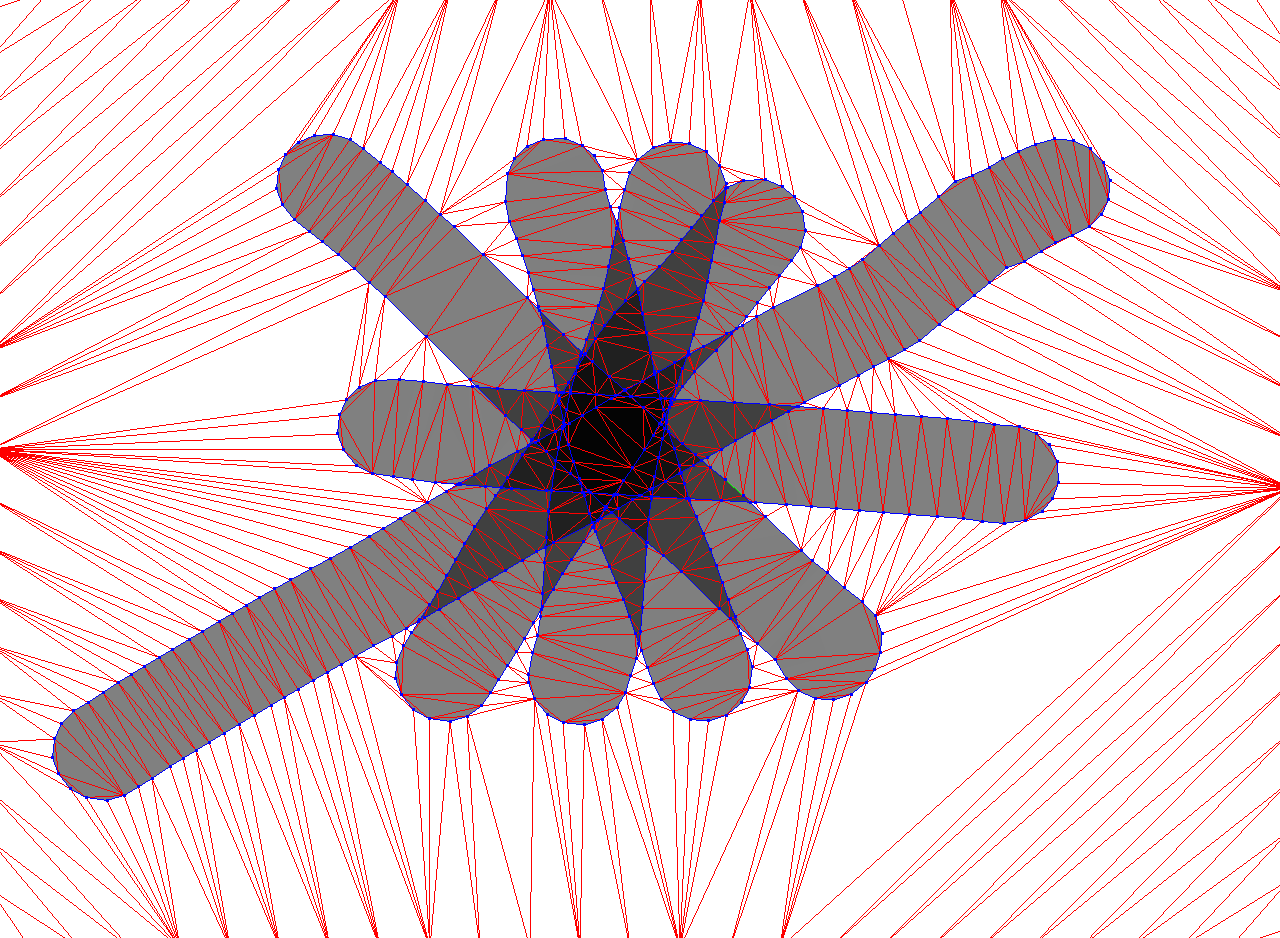
\includegraphics[height=1.5in]{images/tri1164points631edges713}

% The complexity of the triangles increase slightly more than linearly since extra points and 
% boundaries are made when boundaries intersect.

% NOTES: 

% -Maybe do the same analysis with soft strokes

% -Look at the time it takes to render these strokes

% -Then show more robust drawings and the number of triangles, points, and boundaries

% -Talk about future work in the conclusion

% - Switch 6.3 and 6.4
\begin{figure*}
    \centering
        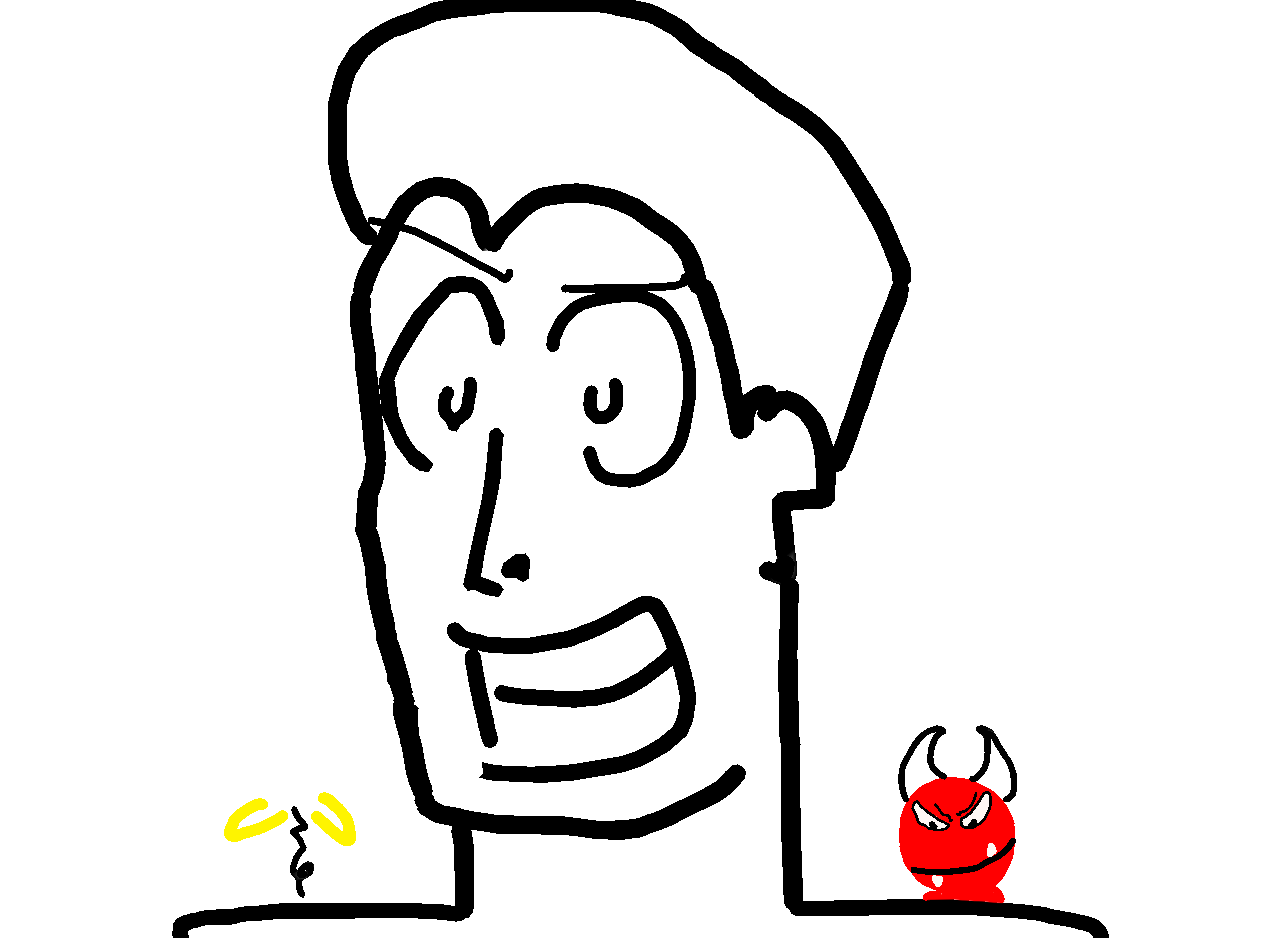
\includegraphics[width=0.49\textwidth]{images/facezoom}
        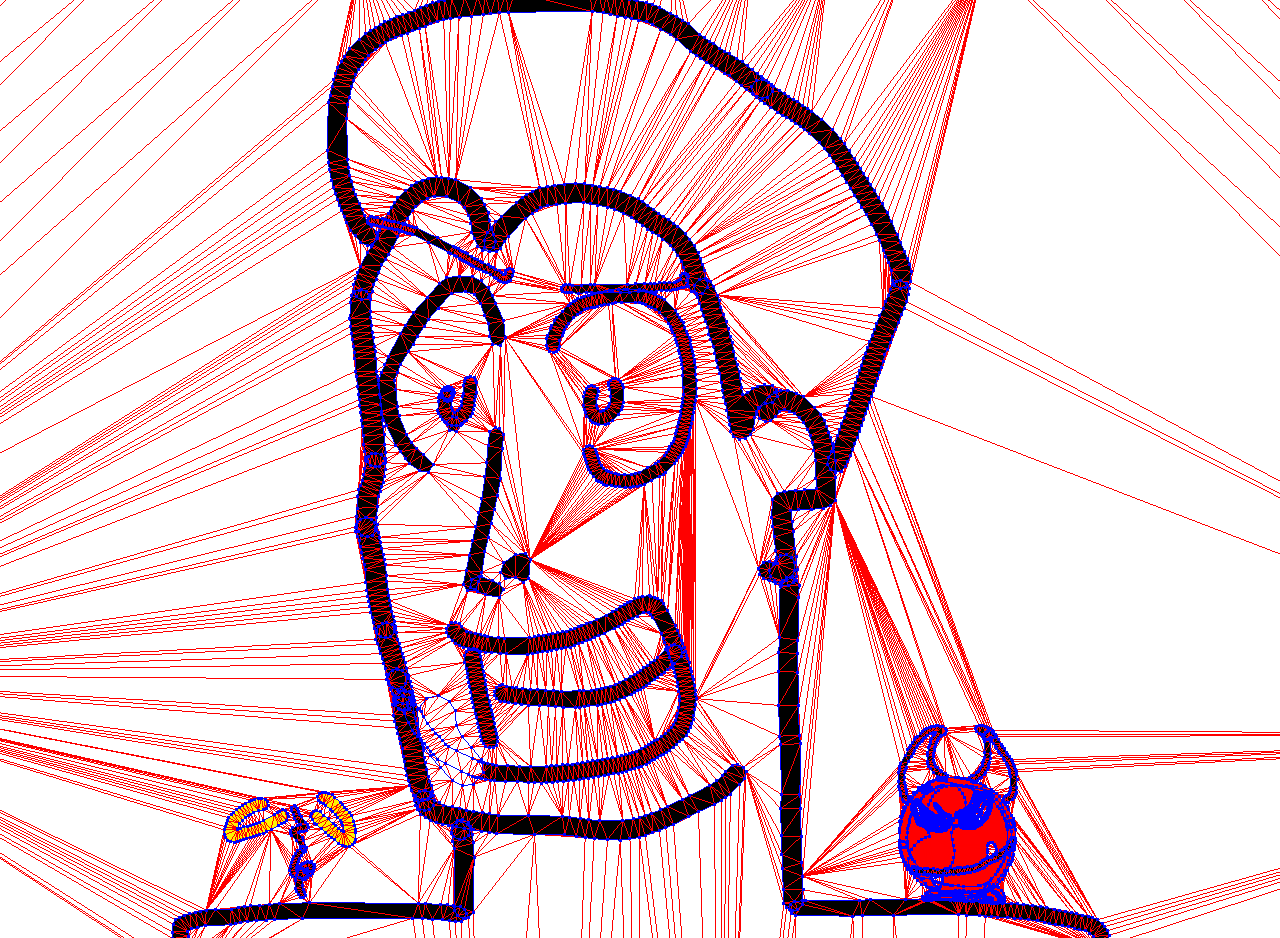
\includegraphics[width=0.49\textwidth]{images/facezoomtriangles}
    \caption{A drawing by an artist that took ~30 minutes. 9030 triangles.} % \Steve{Can we add number of strokes?}}
    \label{fig:face}
\end{figure*}

\begin{figure*}
    \centering
        
\includegraphics[width=0.3\textwidth]{images/stop12}
        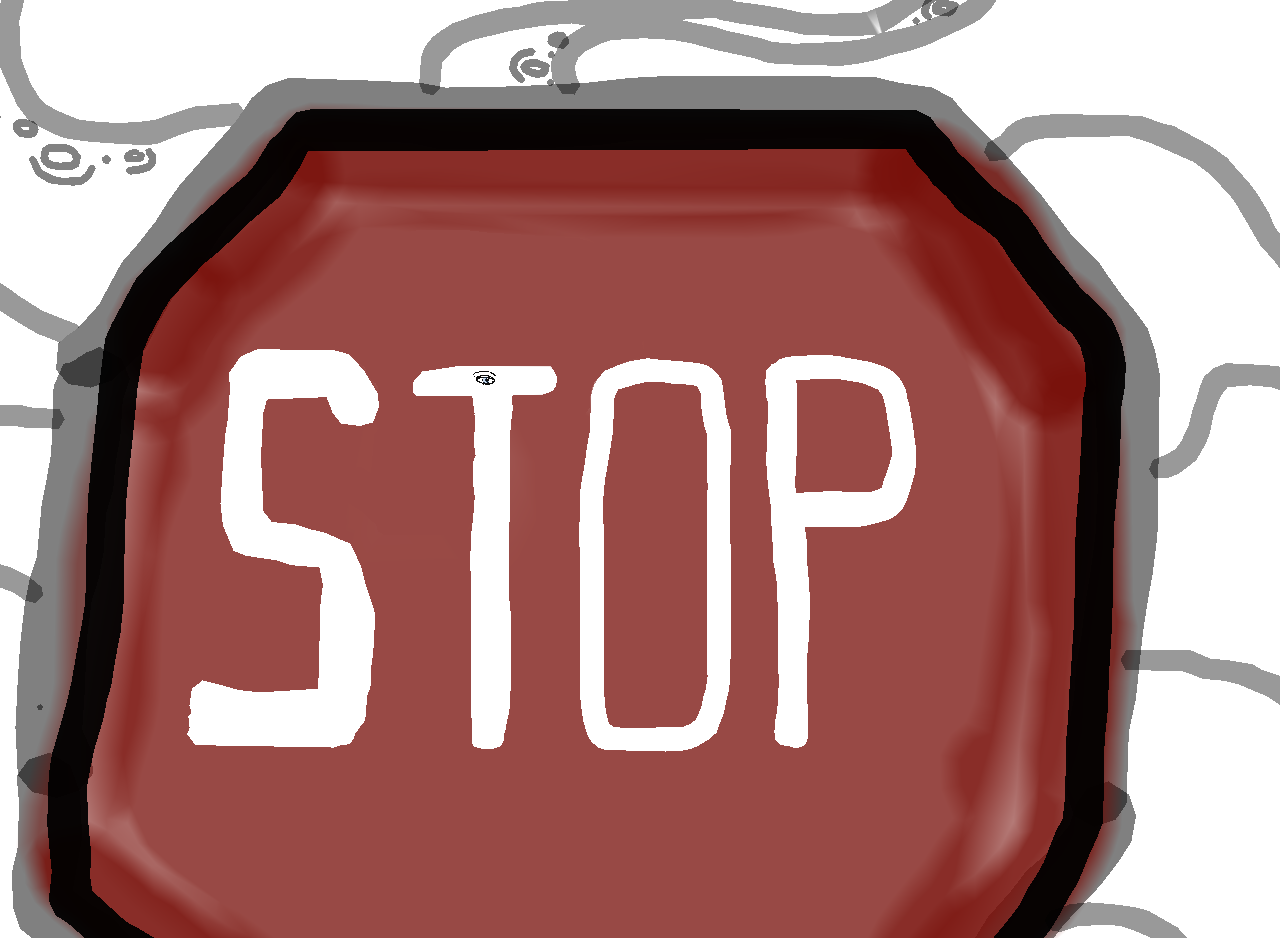
\includegraphics[width=0.3\textwidth]{images/stop22}
        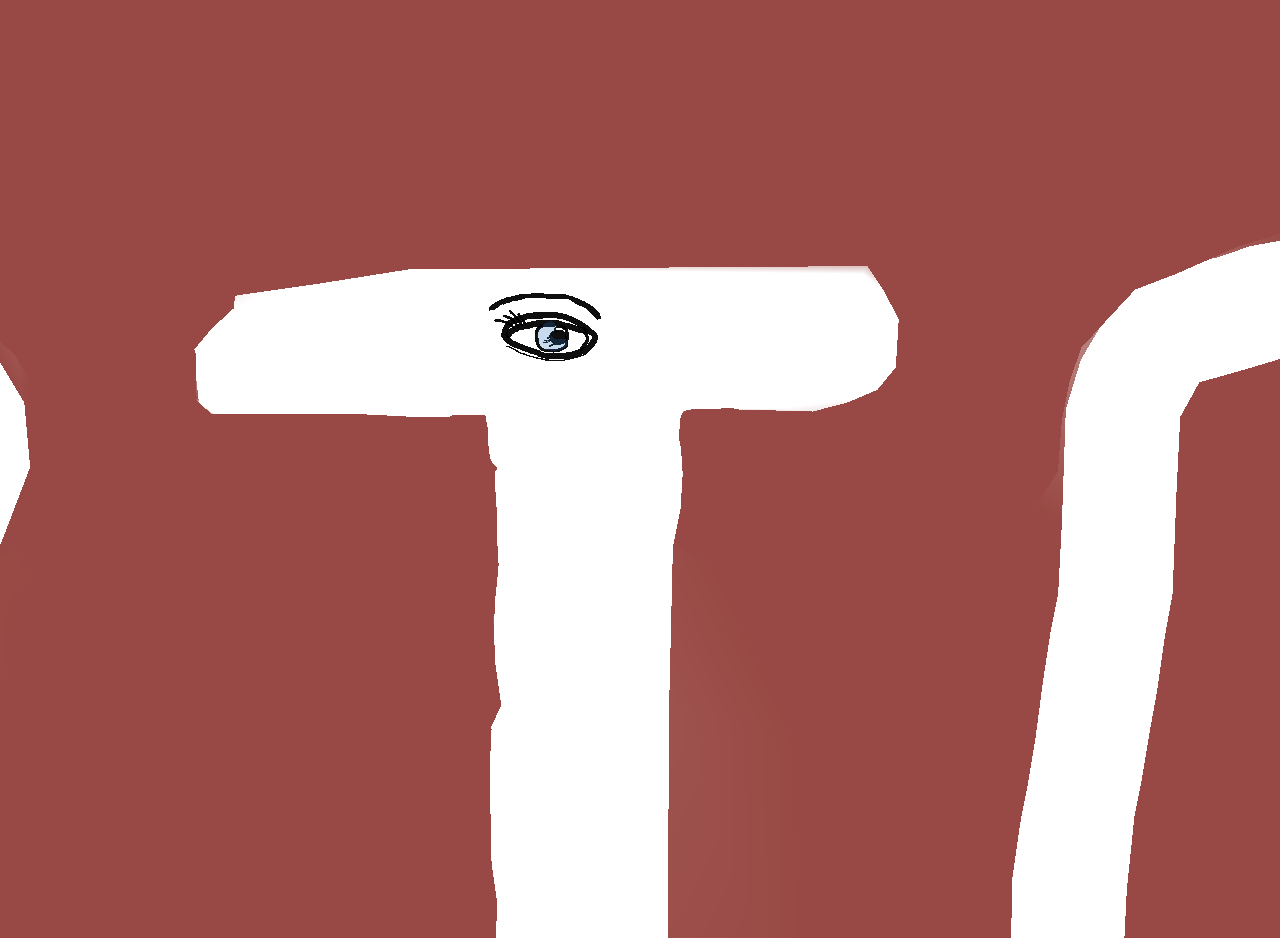
\includegraphics[width=0.3\textwidth]{images/stop32}
    \caption{Another painting by an artist, using soft and hard strokes at a variety of scales.  Middle and right images are zoomed in.}
    \label{fig:stop}
\end{figure*}


\begin{figure*}
    \centering
        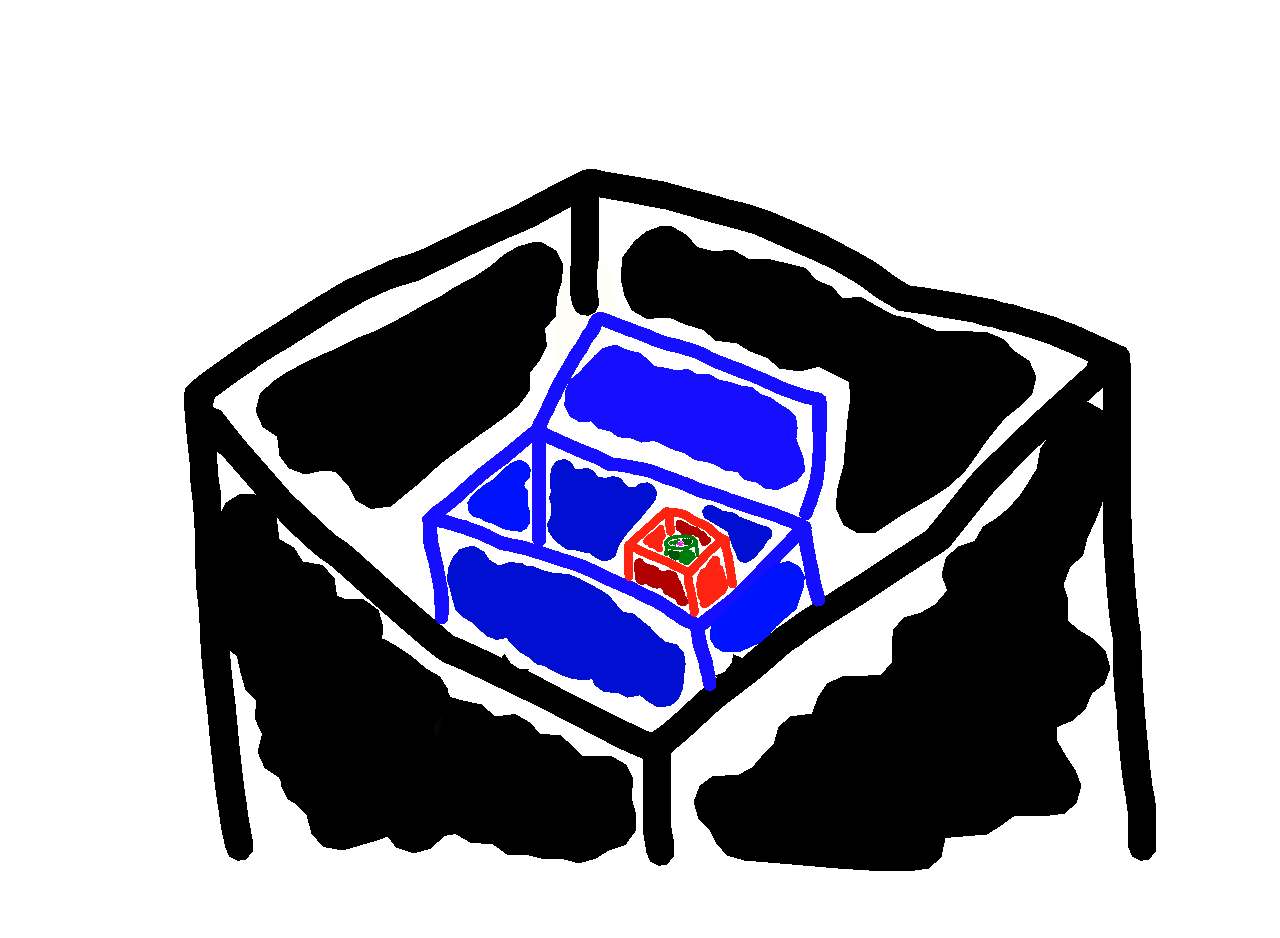
\includegraphics[width=0.195\textwidth]{images/zoom61}
        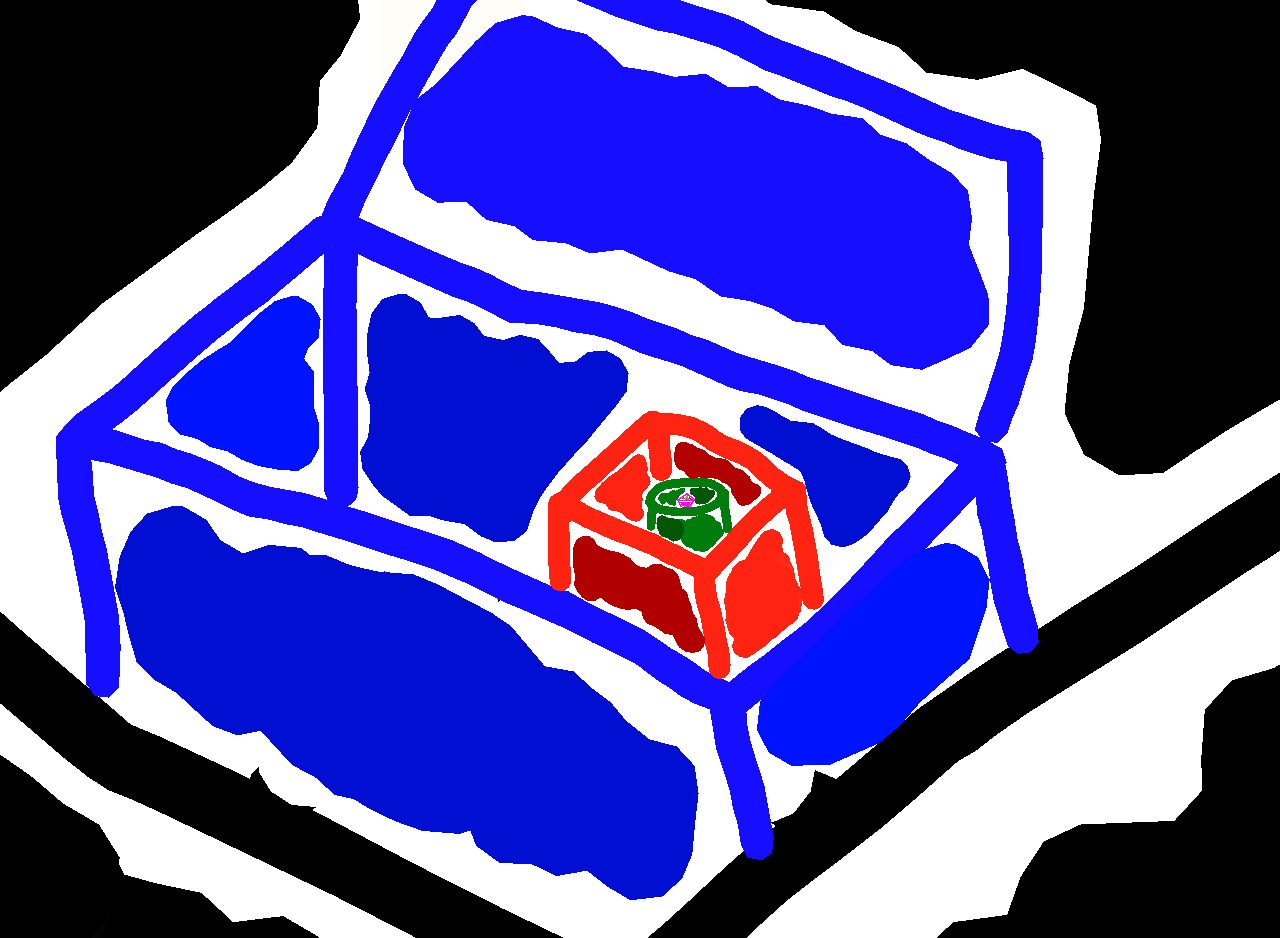
\includegraphics[width=0.195\textwidth]{images/zoom62}
        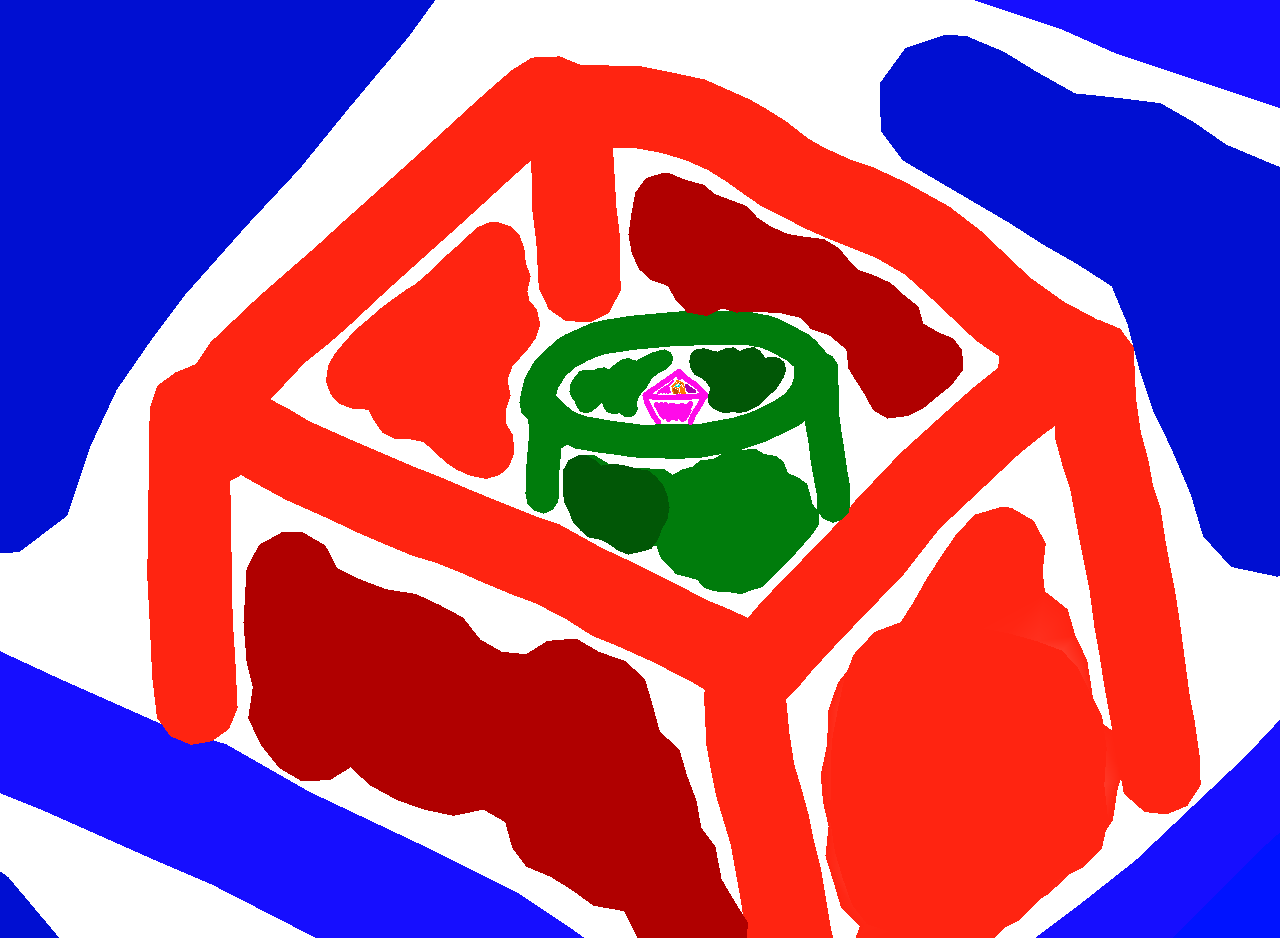
\includegraphics[width=0.195\textwidth]{images/zoom63}
        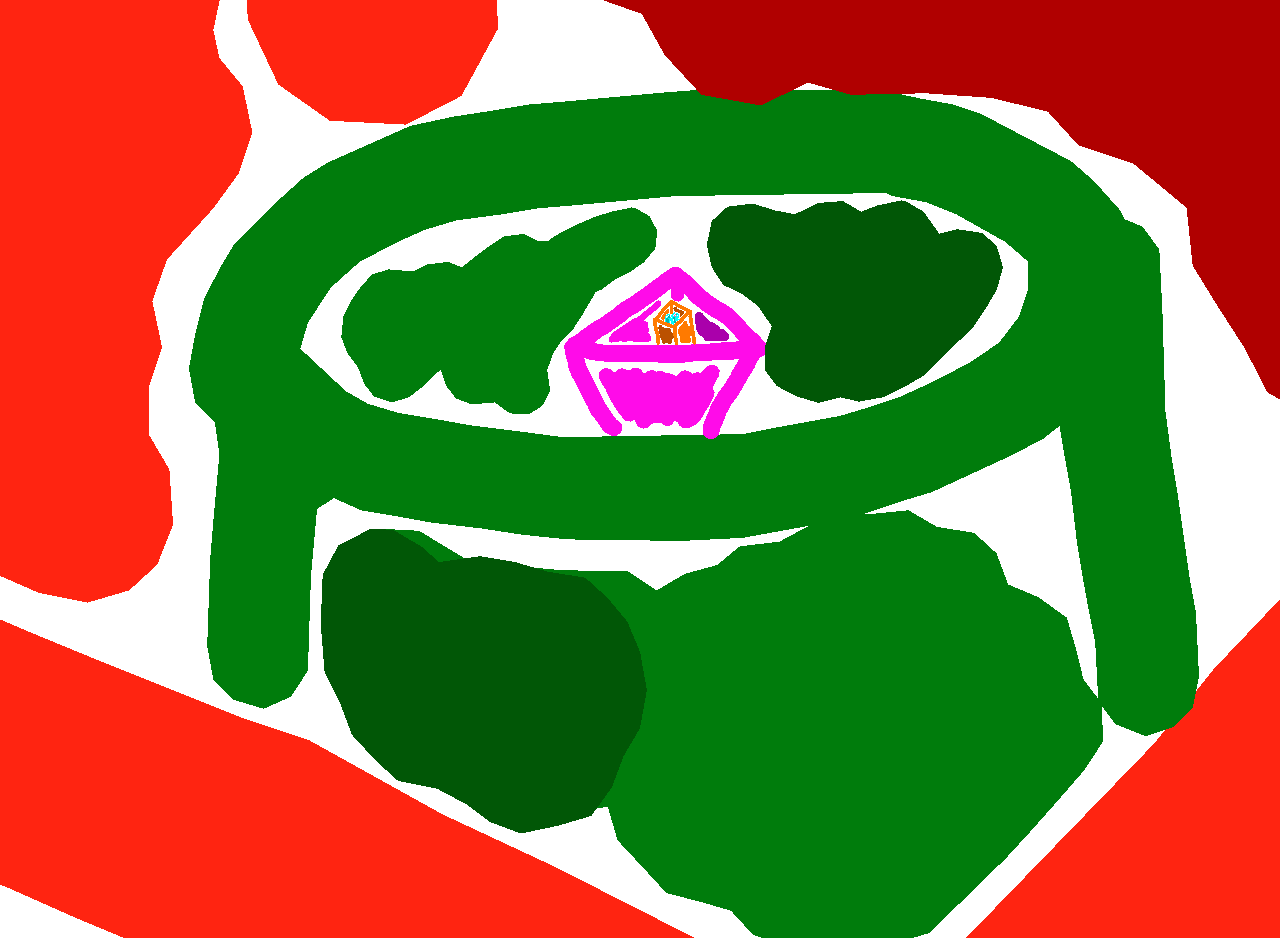
\includegraphics[width=0.195\textwidth]{images/zoom64}
        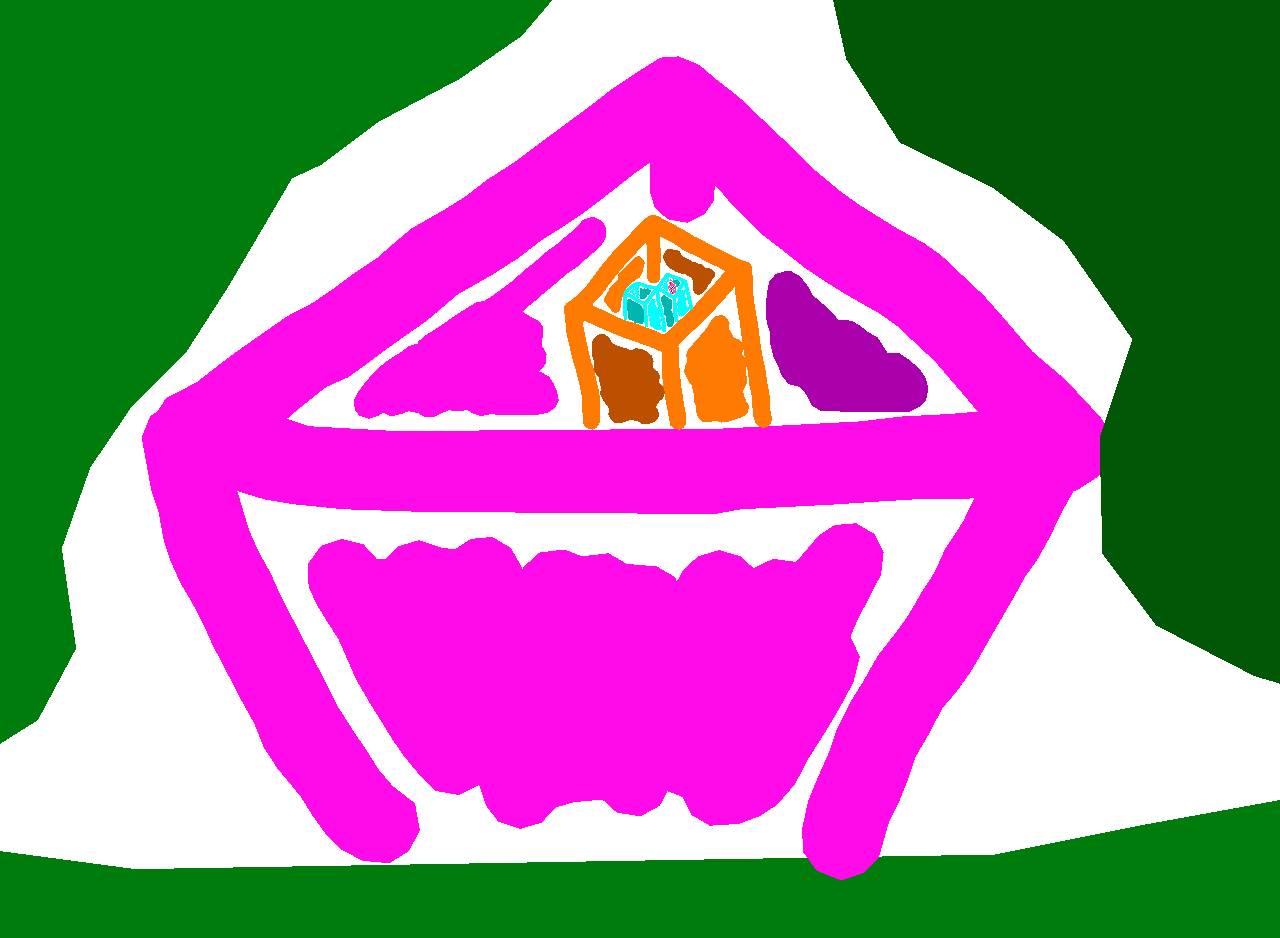
\includegraphics[width=0.195\textwidth]{images/zoom65}
        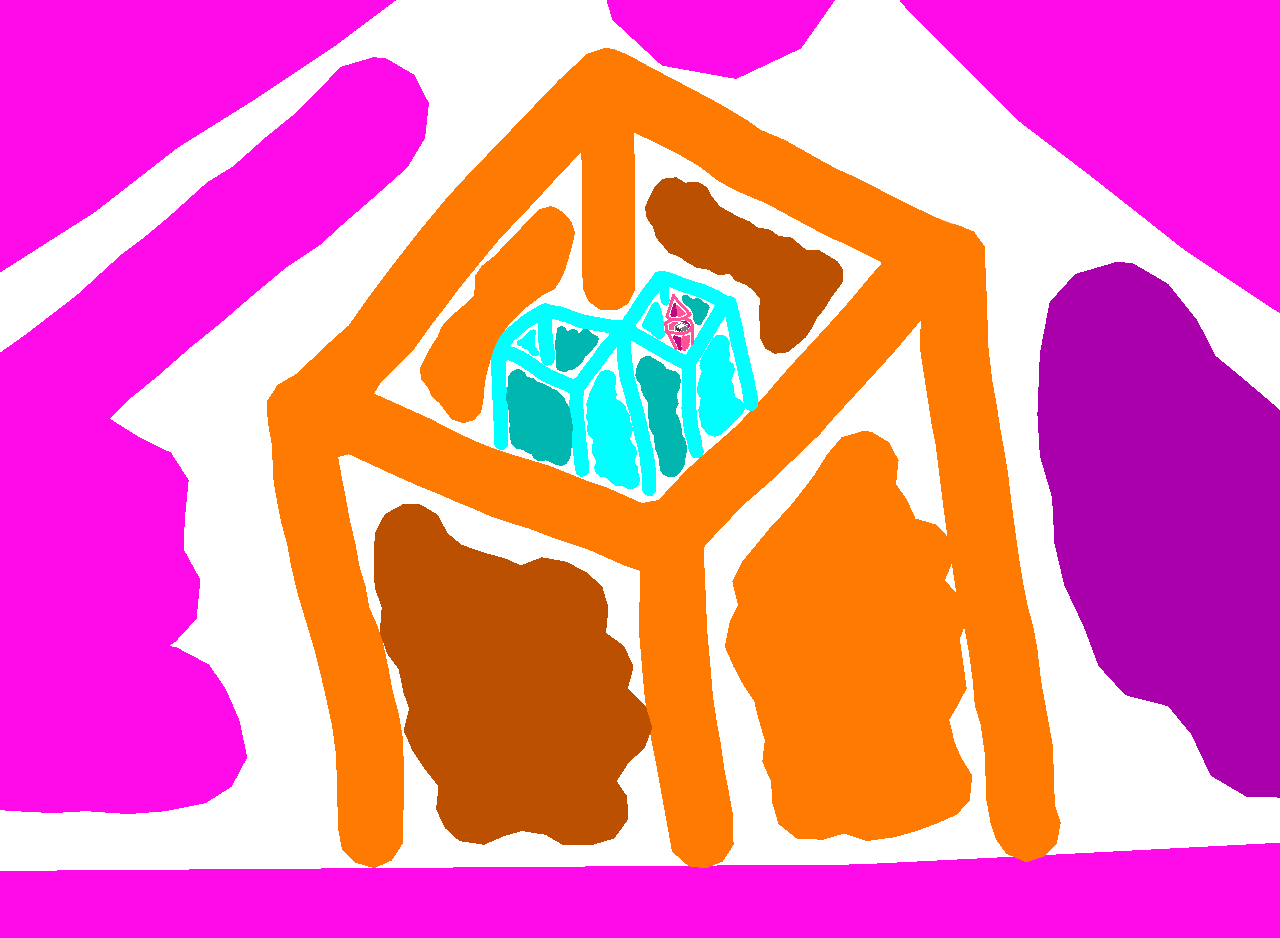
\includegraphics[width=0.195\textwidth]{images/zoom66}
        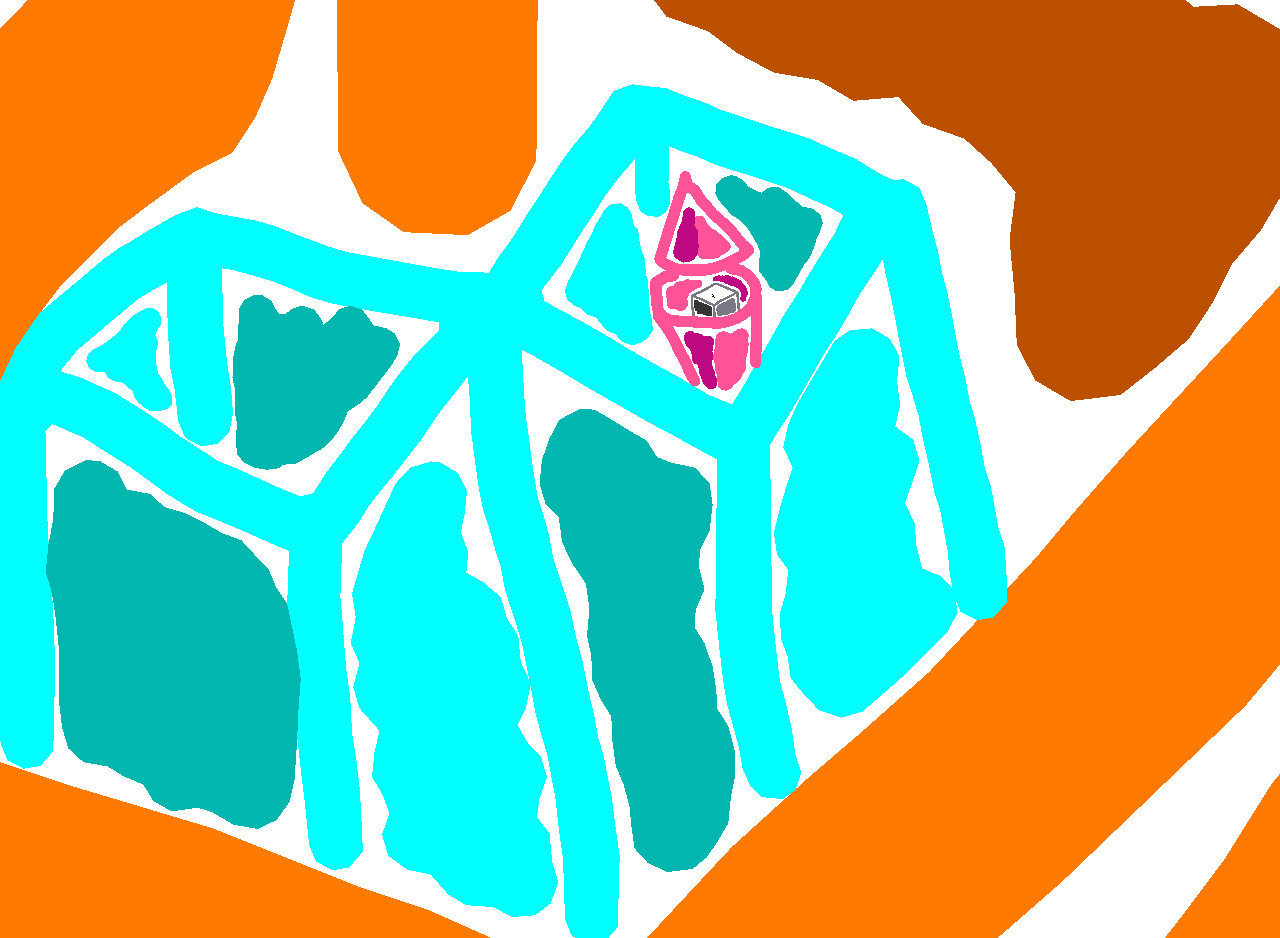
\includegraphics[width=0.195\textwidth]{images/zoom67}
        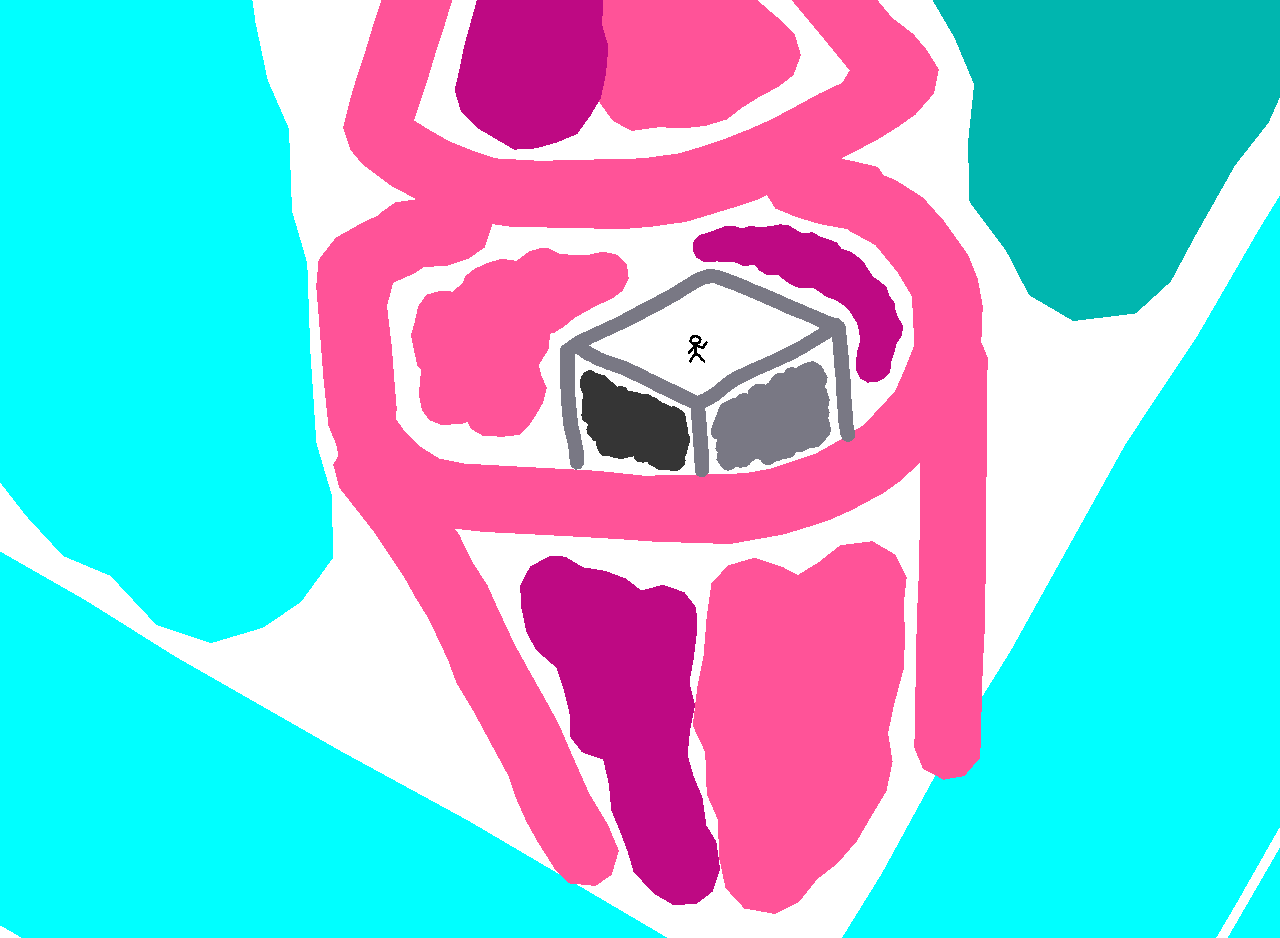
\includegraphics[width=0.195\textwidth]{images/zoom68}
        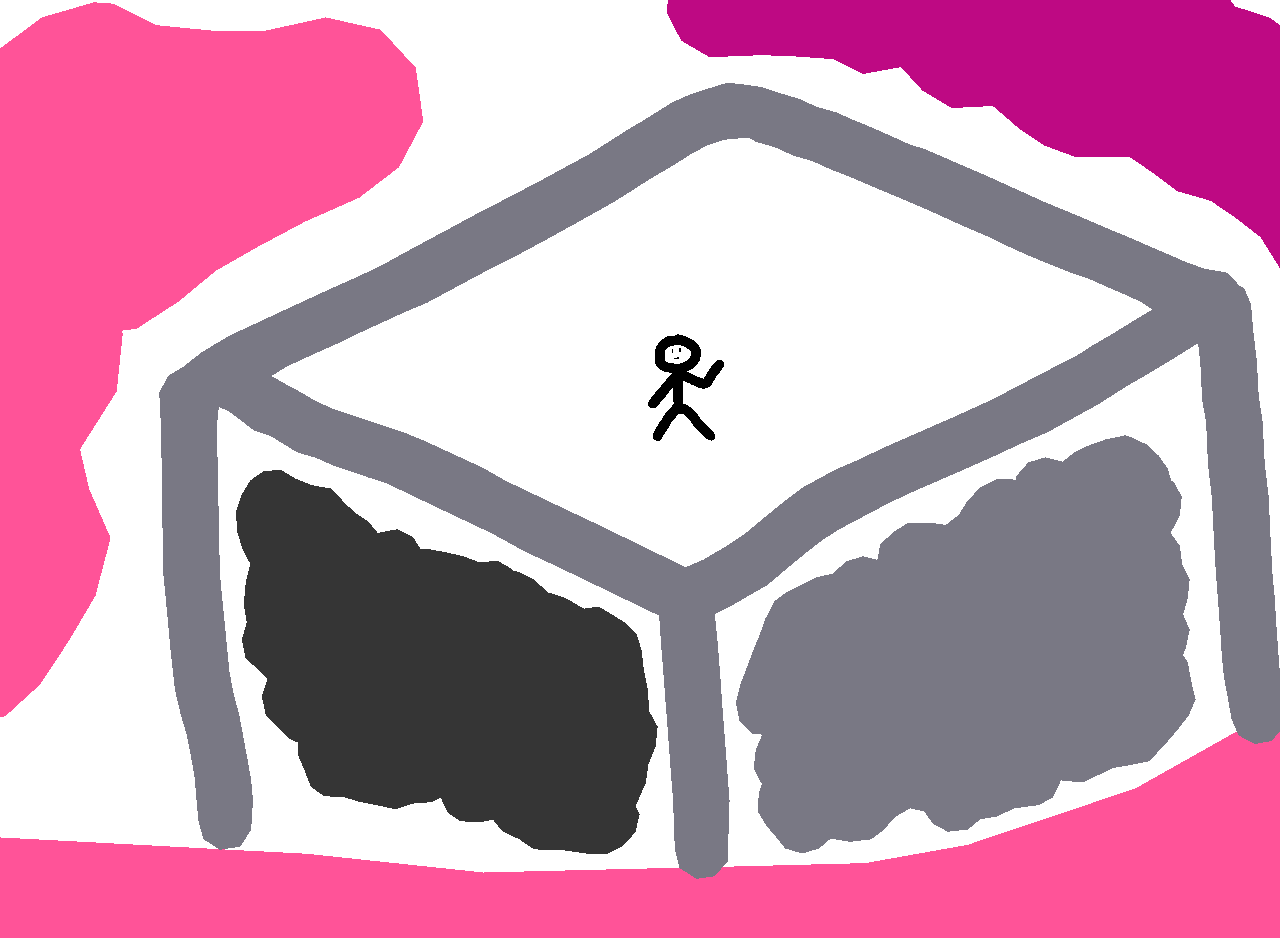
\includegraphics[width=0.195\textwidth]{images/zoom69}
        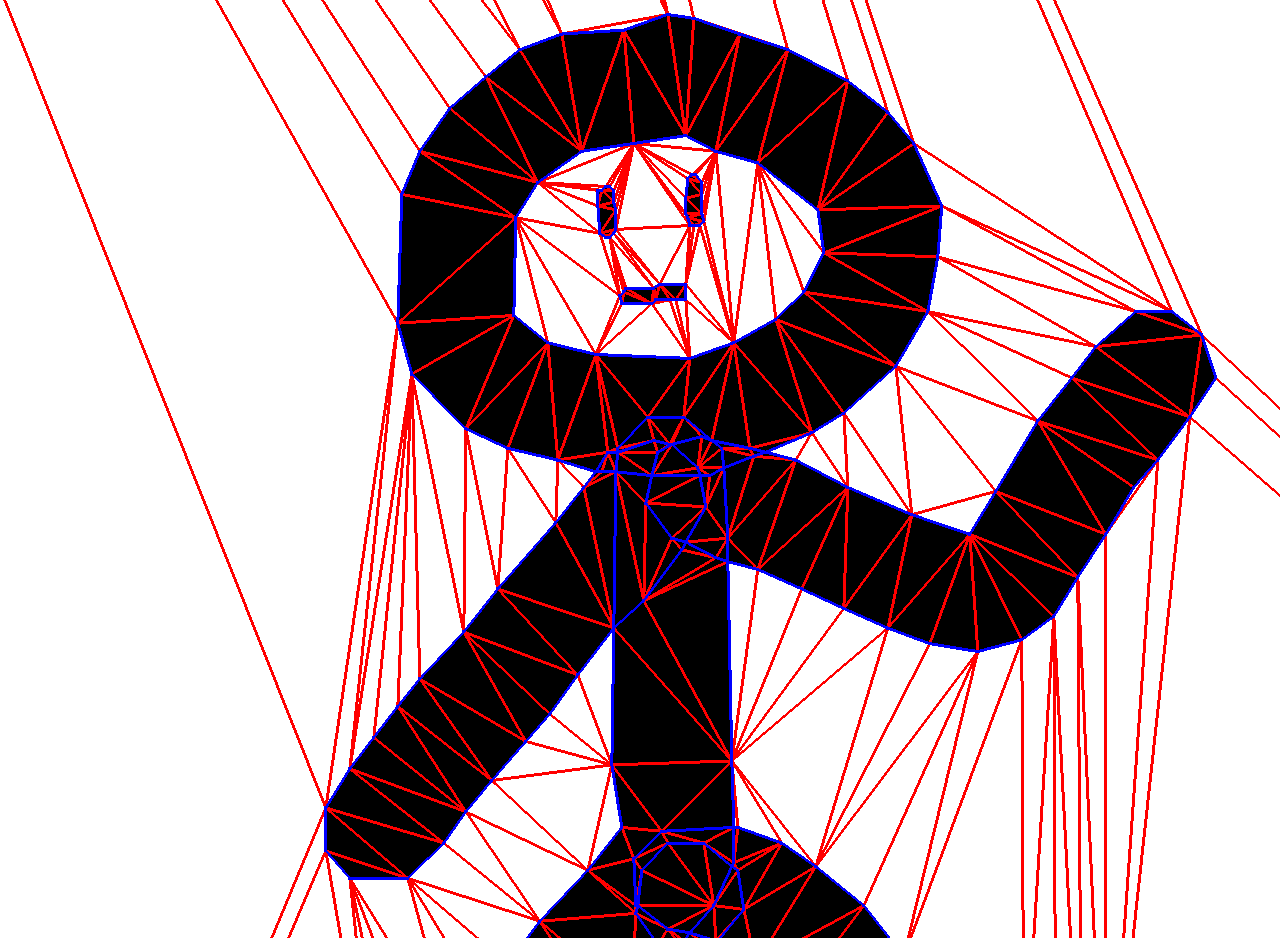
\includegraphics[width=0.195\textwidth]{images/zoom72}
    \caption{A painting that shows extreme zoom levels.  The final image is at zoom level 524,000.}
    \label{fig:boxes}
\end{figure*}

\section{Conclusion}
The system enables a user to paint like they would in a raster graphics program 
to create vector graphics. The core of the system is a triangle mesh representation of the image.
We have created an algorithm to convert a user's mouse motions into a triangle mesh, and then composite
that mesh on the preexisting mesh containing the previous strokes.

The current implementation provides a baseline painting experience. Future work should focus on
implementing a simplification algorithm to allow the complexity of the drawings to grow. Other
improvements might focus on creating interesting manipulation tools, or other operations that utilize
the underlying triangle mesh structure to make the artists' job easier.


\section*{Acknowledgments}

Omitted for review.

\bibliographystyle{acmsiggraph}
\bibliography{paper}
\end{document}
